%------------------ vorlage.tex ------------------------------------------------
%
% LaTeX-Vorlage zur Erstellung von Projektdokumentationen
% im Fachbereich Informatik der Hochschule Trier
%
% Basis: Vorlage 'svmono' des Springer Verlags
% Bearbeiter: Hermann Schloß, Christian Bettinger
%
%-------------------------------------------------------------------------------


%------------------ Präambel ---------------------------------------------------
\documentclass[envcountsame, envcountchap, deutsch]{i-studis}

\usepackage{titlesec}

\usepackage[utf8]{inputenc}

\usepackage[a4paper]{geometry}
\usepackage[english, ngerman]{babel}

\usepackage[pdftex]{graphicx}
\usepackage{epstopdf}

\usepackage{listings}

\usepackage[german, ruled, vlined]{algorithm2e}
\usepackage{amssymb, amsfonts, amstext, amsmath}
\usepackage{array}
\usepackage[skip=10pt]{caption}
\usepackage[usenames, dvipsnames]{color}
\usepackage[pdftex, plainpages=false]{hyperref}
\usepackage{textcomp}

\usepackage{bibgerm}
\bibliographystyle{geralpha}

\usepackage{makeidx}
\usepackage{multicol}
\makeindex

\pagestyle{myheadings}
\setlength{\textheight}{1.1\textheight}

% My Packages
% Tabelle über mehrere Seiten
\usepackage{longtable}
% kursive Captions
\usepackage[font=md,labelfont=it]{caption}

\usepackage[bottom]{footmisc}

\usepackage[framemethod=tikz]{mdframed}
\usepackage{hyperref}
\usepackage{bm}
\usepackage{enumitem}

\usepackage{listings} 			% Code-Darstellung
\lstset{
	%basicstyle=\scriptsize\ttfamily,
	%commentstyle=\scriptsize\ttfamily\color{Gray},
	%identifierstyle=\scriptsize\ttfamily,
	%keywordstyle=\scriptsize\ttfamily,
	%stringstyle=\scriptsize\ttfamily,
	tabsize=4,
	%numbers=left,
	%numberblanklines=false,
	frame=single,
	framesep=3mm,
	framexleftmargin=7mm,
	xleftmargin=10mm,
	linewidth=144mm,
	captionpos=t,
	% my stuff
	lineskip=6.0pt
}

% escape \n characters
\newcommand*{\escape}[1]{\texttt{\expandafter\string\csname #1\endcsname}}

% configuration file for environments
% Listings
\definecolor{dkgreen}{rgb}{0,0.6,0}
\definecolor{gray}{rgb}{0.5,0.5,0.5}
\definecolor{mauve}{rgb}{0.58,0,0.82}
% \definecolor{custom}{rgb}{0.07,0,1}
% \definecolor{custom}{rgb}{0.82,0.54,0.44}
\definecolor{strings}{rgb}{0.71,0,0.04}
% \definecolor{keywords}{rgb}{0.22,0.58,0.80}
\definecolor{keywords}{rgb}{0.14,0.00,1.00}
% \definecolor{ndkeywords}{rgb}{0.82,0.51,0.77}
\definecolor{ndkeywords}{rgb}{0.75,0.00,0.89}
\lstdefinelanguage{JavaScript}{
  keywords={typeof, new, true, false, catch, async, function, return, null, catch, switch, var, let, const, if, in, while, do, else, case, break},
  keywordstyle=\color{keywords}\bfseries,
  ndkeywords={class, export, boolean, throw, implements, import, this, await},
  ndkeywordstyle=\color{ndkeywords}\bfseries,
  identifierstyle=\color{black},
  sensitive=false,
  comment=[l]{//},
  morecomment=[s]{/*}{*/},
  commentstyle=\color{purple}\ttfamily,
  stringstyle=\color{strings}\ttfamily,
  morestring=[b]',
  morestring=[b]"
}

\lstdefinestyle{basiccode}{
  basicstyle=\ttfamily,
  columns=fullflexible,
  gobble=2,
  xleftmargin=.1in,
  framexleftmargin=.05in,
  xrightmargin=.12in,
  framextopmargin=.05in,
  framexbottommargin=.04in,
  escapechar=~
}

\lstnewenvironment{basiccode}
{\lstset{style=basiccode}}
{}

\lstnewenvironment{javascript}[2]
{\lstset{
  style=basiccode,
  frame=tblr,
  language=JavaScript,
  aboveskip=3mm,
  belowskip=3mm,
  showstringspaces=false,
  columns=flexible,
  basicstyle={\small\ttfamily},
  numbers=none,
  numberstyle=\tiny\color{gray},
%   keywordstyle=\color{blue},
%   commentstyle=\color{dkgreen},
%   stringstyle=\color{mauve},
  breaklines=true,
  breakatwhitespace=true,
  tabsize=3,
  escapechar=~,}
}
{%
    \captionof{lstlisting}{#1}
    \label{#2}
}



%------------------ Manuelle Silbentrennung ------------------------------------
\hyphenation{Ele-men-tar-ob-jek-te ab-ge-tas-tet Aus-wer-tung House-holder-Matrix Least-Squares-Al-go-ri-th-men kom-plex-er}


%------------------ Titelseite -------------------------------------------------
\begin{document}

\title{\textbf{gedcom7.js}}
\subtitle{Realization of a JavaScript Library for the Genealogical Exchange Format FamilySearch GEDCOM Version 7}
\subtitle{Realisierung einer JavaScript-Bibliothek für das genealogische Austauschformat FamilySearch GEDCOM Version 7}


\author{Marius Müller \& David Gruber}

\supervisor{Christian Bettinger}

\address{Trier}
\submitdate{28.02.2023}

%------------------ Projektart -------------------------------------------------
\project{Bachelor-Projektarbeit}
%\project{Bachelor-Abschlussarbeit}
%\project{Master-Projektstudium}
%\project{Master-Abschlussarbeit}
%\project{Seminararbeit}
%\project{Hausarbeit}

\mytitlepage

%------------------ Vorwort, Kurzfassung, Verzeichnisse ------------------------
\frontmatter
%\input{chapters/Vorwort}								% Vorwort (optional)
\kurzfassung
In dieser Arbeit wurde die JavaScript-Bibliothek \textit{gedcom7.js} für das genealogische Austauschformat FamilySearch GEDCOM Version 7 entwickelt und getestet. Das grundlegende Element der Bibliothek stellt dabei ein Parser dar, der Dateien im Format Gedcom7 lesen und schreiben kann. Beim Lesen wird der Inhalt der Datei, nach der in der Gedcom7 Spezifikation definierte Syntax überprüft und in geeignete Datenstrukturen überführt. Diese Datenstrukturen stellen Funktionalitäten zu Veränderung und Erweiterung der Dateien bereit. Bei allen Operationen finden Syntaxüberprüfungen statt, sodass zu jedem Zeitpunkt garantiert ist, dass eine Gedcom7-konforme Struktur vorliegt. Der Hauptfokus der Implementierung liegt auf einfacher Erweiterbarkeit, weshalb ein Grammatik Generator entwickelt wurde, der die Grammatiken zur Syntaxüberprüfung automatisiert generiert.

\kurzfassungEN
In this work, the JavaScript library  gedcom for the genealogical exchange format FamilySearch GEDCOM Version 7 was developed and tested. The basic element of the library is a parser that can read and write files in the Gedcom7 format. During reading, the content of the file is checked according to the syntax defined in the Gedcom7 specification and converted into suitable data structures. These data structures provide functionalities for changing and expanding the files. Syntax checks are performed in all operations, so that a Gedcom7-compliant structure is guaranteed at all times. The main focus of the implementation is on easy extensibility, which is why a grammar generator has been developed that automatically generates grammars for syntax checking.
							% Kurzfassung/Abstract
\tableofcontents										% Inhaltsverzeichnis
\listoffigures											% Abbildungsverzeichnis (optional)
%\listoftables											% Tabellenverzeichnis (optional)
%\lstlistoflistings										% Listings (optional)


%------------------ Kapitel ----------------------------------------------------
\mainmatter
\chapter{Einleitung und Problemstellung}
\label{chap: Einleitung und Problemstellung}
In dieser Ausarbeitung ...

\section{Anforderungsanalyse \& Ziele}
\label{Anforderungsanalyse und Ziele}
Folgende Anforderungen werden an die Bibliothek gestellt: 
\begin{itemize}
	\item AF01: Dateien oder Strings im Format Gedcom7 sollen eingelesen werden können
	\item AF02: Dateien sollen im Gedcom7 Format ausgegeben werden können 
	\item AF03: Die Syntax von Dateien oder Strings soll gemäß der Gedcom7-Spezifikation überprüfbar sein 
	\item AF04: Die in der Gedcom7-Spezifikation definierten Datentypen sollen unterstützt werden 
	\item AF05: Eingelesene Dateien sollen gemäß der Gedcom7-Spezifikation verändert und erweitert werden können
	\item AF06: Die Bibliothek soll erweiterbar sein  
\end{itemize}

\chapter{Theoretische Grundlagen}
\label{chap: Theoretische Grundlagen}
In diesem Kapitel werden die theoretischen Grundlagen für das Verständnis dieser Projektarbeit beschrieben. Dazu wird eine kurze Einführung in Genealogie, FamilySearch und GEDCOM im speziellen gegeben, um ein Verständnis für die Thematik aufzubauen. Zudem wird auf mehrere Quellen verwiesen, aus denen tiefergehende Informationen erschlossen werden können. Im Anschluss dazu wird kurz auf die JavaScript Bibliothek \textit{Nearley} und das JavaScript Testframework \textit{Mocha} eingegangen, die für die Umsetzung dieser Projektarbeit relevant werden.

\section{Genealogie und FamilySearch}
\label{sec: Genealogie und FamilySearch}
Genealogie ist ein Überbegriff für die Familien- und Ahnenforschung und beschäftigt sich mit der historischen Herkunft und der Geschichte von Menschen weltweit \cite{AhnenforschungDE}. Dabei sind insbesondere Abstammungs- und Verwandtschaftsverhältnisse von besonderer Bedeutung, die anhand von Beiweisen aus validen Quellen in Stammbäumen zusammengefasst werden, die aufzeigen, wie eine Generation mit der nächsten verbunden ist. Auf Basis der so erlangten Erkenntnisse kann eine Familiengeschichte erstellt werden, die eine biographische Studie einer genealogisch nachgewiesenen Familie und der Gemeinde in der sie lebten, darstellt \cite{SocietyOfGenealogists}.

Das Aufkommen des Internets stellte einen Wendepunkt in der Genealogie dar. Die einfachere Kommunikation auch über Landesgrenzen hinweg, ermöglicht es genealogische Informationen auszutauschen und so Gleichgesinnte und Verwandte auf der ganzen Welt zu finden \cite{AhnenforschungDE}. Um einen standardisierten Austausch genalogischer Informationen zu ermöglichen, entwickelte die Kirche Jesu Christi der Heiligen der Letzten Tage das Datenformat GEDCOM, das im folgenden Kapitel vorgestellt wird.
\newpage
\section{GEDCOM Version 7}
{
\label{sec: GEDCOM Version 7}
Das Datenformat FamilySearch GEDCOM 7.0 ist ein einheitliches, flexibles Format für den Austausch von genealogischen Daten, das 2021 von der Kirche Jesu Christi der Heiligen der Letzten Tage entwickelt wurde. Das Ziel besteht darin, eine langfristige Speicherung von genealogischen Informationen zu ermöglichen, die für zukünftige Genealogen und die von ihnen verwendeten System zugänglich und verständlich sind \cite{GEDCOM}. Die im Rahmen dieser Arbeit verwendete Version 7.0.11 wurde am 01.11.2022 veröffentlicht und stellt die aktuelleste Version des Standards dar\footnote{Stand 31.01.2023}. 

GEDCOM ist ein UTF-8 kodiertes hierarchisches Containerformat, das die Dateinamenserweiterung \textit{.ged} verwendet. Der erste Character einer GEDCOM-Datei sollte das Byte-Order-Mark (U+FEFF) sein. Der Inhalt einer GEDCOM-Datei ist in sog. \textit{Structures} unterteilt, die aus einem \textit{Structure-Type} und einem optionalen \textit{Payload} bestehen und mehrere Substrukturen besitzen können. Hat eine \textit{Structure} eine \textit{Substructure}, dann ist die \textit{Structure} die \textit{Superstructure} der \textit{Structure}. Jede \textit{Substructure} hat genau eine \textit{Superstructure} und ist so eindeutig zugeordnet. Eine \textit{Structure}, die keine \textit{Supertructure} besitzt, heißt \textit{Record}. Alle Records zusammen mit einem Header und einem Trailer bilden ein \textit{Dataset}, das den Inhalt einer GEDCOM-Datei darstellt. \cite{GEDCOM} 

Der \textit{Payload} einer \textit{Structure} ist eine Zeichenkette eines bestimmten Datentyps, die entweder Informationen für die \textit{Supertructure} bereithält, oder einen Zeiger auf eine andere \textit{Structure} repräsentiert und somit auf diese verweist. GEDCOM v7 definiert 11 verschiedene Datentypen in \cite{GEDCOM} mit denen Namen, Daten, Uhrzeiten, Texte und vieles mehr dargestellt werden können. Der \textit{Structure-Type} ist eindeutig definiert durch eine URI und gibt an, welche Bedeutung und welchen Datentyp die \textit{Structure} besitzt, welche \textit{Substructures} enthalten sein können und mit welcher Kardinalität diese auftreten können. \cite{GEDCOM} 

Kodiert wird der Inhalt einer GEDCOM-Datei in sog. \textit{Lines}, die eine Zeichenkettenrepräsentation einer \textit{Structure} (bzw. eines Teils einer \textit{Structure}) darstellen und wie in Listing \ref{lst: gedcom line} aufgebaut sind. Die Bedeutung der einzelnen Bestandteile einer Line ist in Tabelle \ref{tab: gedcom line} spezifiziert.
\vspace{1em}
\begin{lstlisting}
	Level  D  [Xref  D]  Tag  [D  LineVal]  EOL
\end{lstlisting}
\captionof{lstlisting}{Aufbau einer GEDCOM Line. Eckige Klammern repräsentieren optionale Inhalte.}
\label{lst: gedcom line}
\newpage
\bgroup
\def\arraystretch{1.5}%  1 is the default, change whatever you need
\setlength{\tabcolsep}{18pt}
\begin{longtable}{|p{2cm}|p{10cm}|}
	\hline
	\textbf{URI} & Eine Line beginnt mit einem Level, das die Verhältnisse der \textit{Structures} untereinander beschreibt. Alle \textit{Structures} mit dem kleinstmöglichen Level $0$ sind Records - Level $\ge1$ repräsentieren \textit{Substructures}. Eine \textit{Structure} mit dem Level $x$ ist also die \textit{Superstructure} aller folgenden \textit{Structures} mit dem Level $x+1$. \\
	\hline
	\textbf{D} & \textit{D} steht für \textit{Delimiter}, was englisch für Trennzeichen ist und repräsentiert in diesem Fall das Leerzeichen mit dem Unicode $u+0020$. \\
	\hline
	\textbf{Xref} & Xref ist die Abkürzung für \textit{Cross-Reference Identifier} und fungiert als Adresse für eine \textit{Structure}. Möchte man von einer \textit{Structure} auf eine andere \textit{Structure} verweisen, kann dies über einen Zeiger-Payload auf die entsprechende \textit{Structure} realisiert werden.\\
	\hline
	\textbf{Tag} & Der \textit{Tag} kodiert den \textit{Structure-Type} einer \textit{Structure}.\\
	\hline
	\textbf{LineVal} & Im \textit{LineVal} einer Struktur ist der Payload kodiert.\\
	\hline
	\textbf{EOL} & EOL steht für End-Of-Line und kodiert das Ende einer Line. Im Format GEDCOM v7 kann dies entweder durch einen Carriage-Return (Unicode U+000D), Line-Feed(Unicode U+000A) oder einen Carriage-Return gefolgt von einem Line-Feed repräsentiert werden.\\
	\hline
	\caption{Bestandteile einer GEDCOM Line und ihre Bedeutung} % needs to go inside longtable environment
	\label{tab: gedcom line}
\end{longtable}
\egroup
\vspace{1em}
Ein Ausschnitt aus einer GEDCOM-Datei ist in Listing \ref{lst: family record example} dargestellt. Dieser Ausschnitt zeigt einen \textit{Record} vom Typ \textit{Family}, in dem Informationen über eine Familie gespeichert werden können. Der Familie wurde der Cross-Reference Identifier \textit{@F1@} zugewiesen, sodass im Dataset auf dieses verwiesen werden kann. Der Ehemann und die Ehefrau der Familie (engl. Husband und Wife) sind die Individuen \textit{I1} und \textit{I2}, die ebenfalls in der Gedcom7-Datei definiert sind. Dieser Zusammenhang wird über die Cross-Reference Identifier \textit{@I1@} und \textit{@I2@} ausgedrückt. Außerdem wird ein Family-Event, nämlich die Hochzeit der beiden Ehepartner, aufgeführt und auf den 1.März 1951 datiert. Als letzte Information ist die Anzahl der Kinder (NCHI: Number of Children) mit 2 spezifiziert.
\newpage
\begin{lstlisting}
	0 @F1@ FAM
	1 HUSB @I1@
	1 WIFE @I2@
	1 MARR
	2 DATE 1 MAR 1951
	1 NCHI 2
\end{lstlisting}
\captionof{lstlisting}{Beispiel für einen Family Record}
\label{lst: family record example}
\vspace{1em}
Detaillierte Erklärungen, alle Informationen zu \textit{Structure Types}, Datentypen, usw. und viele weitere Beispiele können in \cite{GEDCOM} nachgelesen werden.
}
\section{Nearley}
\label{sec: Nearley}
% TO-DO: EBNF erklären bzw. einmal ansprechen -> vielleicht schon im Gedcom-Kapitel?
Nearley.js ist eine JavaScript-Bibliothek zum Parsen kontextfreier Grammatiken (CFGs). Sie bietet einen vielseitigen und effizienten Parsing-Algorithmus, 
der auf dem Algorithmus von Earley basiert und es ermöglicht, mehrdeutige und rekursive Grammatiken mit Leichtigkeit zu behandeln. Die Bibliothek ist 
modular aufgebaut, so dass Benutzer ihre eigenen Parser und Lexer definieren und Parser aus externen Quellen wie BNF- und EBNF-Grammatiken erzeugen können. 
Nearley.js ist in reinem JavaScript implementiert und kann in jeder Umgebung ausgeführt werden, die JavaScript unterstützt, einschließlich Webbrowsern und 
serverseitigen Umgebungen.


Nearley.js bietet eine Reihe nützlicher Funktionen, darunter JavaScript-Aktionen, genannt \textit{Postprocessor}, bei denen Benutzer Code angeben können, 
der ausgeführt wird, wenn bestimmte Teile der Eingabe erkannt werden. Nearley.js ist Open-Source und hat eine lebendige Gemeinschaft von Nutzern und 
Mitwirkenden, was es zu einem zuverlässigen und gut unterstützten Werkzeug für das Parsen komplexer Texte macht.


Im Laufe der Implementierung haben wir uns dazu entschieden, die komplette GEDCOM-Grammatik mittels Nearley abzubilden. Dies hat den Vorteil, dass wir 
alle Regeln der GEDCOM-Spezifikation in einer Prüfung abdecken können. Außerdem bietet Nearley die Möglichkeit Teile der Grammatik in einzelnen Dateien
auszulagern und nur für Teile der Grammatik Parser zu erstellen. Dies ermöglicht es uns eine Teilprüfung von nur einer GEDCOM-Struktur einer
ganzen Datei durchzuführen. Dies ist insbesondere bei Manipulationen von einzelnen Strukturen innerhalb einer Datei von Vorteil, da anschließend
nur die betroffene Struktur neu geprüft werden muss.

% TO-DO: Beispiel einer Nearley Grammatik einfügen und erklären

\section{Mocha}
\label{sec: Mocha}

Im Rahmen der Implementierung unserer Bibliothek, war es uns ein zentrales Anliegen, das Testen dieser zu gewährleisten. Zu diesem Zweck haben wir uns auf die Suche nach einem geeigneten Testframework für JavaScript begeben. In diesem Kontext stießen wir auf Mocha, welches eine API bereitstellt, die das einfache Erstellen von Tests ermöglicht. Wie bei vielen anderen Testframeworks können Assertion-Funktionen genutzt werden, um die Tests zu überprüfen.

Wie im Beispiel-Test in Listing \ref{lst: mocha example} veranschaulicht wird, wird zunächst ein aussagekräftiger Name für den Test als erster Parameter der Mocha-Funktion \textit{describe} übergeben. Im zweiten Parameter wird eine Callback-Funktion übergeben, die den Code für den Test enthält, beginnend mit dem Setup-Code. Hierbei wird in unserem Fall ein Array mit mehreren Gedcom-Dateinamen erstellt, die sich im angegebenen \textit{path} befinden.

Durch die Verwendung der Funktion \textit{forEach}, welche aus einem Mocha-Plugin namens \textit{mocha-each} stammt, wird über alle Dateinamen iteriert. Für jeden Dateinamen wird ein neuer Test erstellt und der Code in der anonymen Callback-Funktion für jeden \textit{fileName} im Array \textit{gedFiles} ausgeführt.

Der Ablauf für eine Datei im Listing \ref{lst: mocha example} ist wie folgt: Zunächst wird die Datei mithilfe der asynchronen Helper-Funktion \textit{readGedFile} eingelesen und in der Variable \textit{beforeParsing} gespeichert. Anschließend wird die Datei mit der Funktion \textit{parseString} des Moduls \textit{gedcomParser} als Dataset geparst. Hierbei wird eine Grammatikprüfung durchgeführt und alle Daten aus der Datei sind nach erfolgreicher Prüfung über die Dataset Klasse und deren Methoden zugänglich.

Im nächsten Schritt wird im aktuellen Verzeichnis eine temporäre Datei namens \textit{temp.ged} erstellt und anschließend mit der Funktion 
\textit{dataset.write} mit den eingelesenen Daten des Datasets beschrieben.

Schließlich wird mithilfe der Funktion \textit{expect}, welche aus dem Mocha-Plugin \textit{chai} stammt, überprüft, ob die eingelesene 
Datei und das geschriebene Dataset in der \textit{temp.ged} Datei identisch sind.
\\\\
Der beschriebene Testmechanismus gewährleistet, dass die Daten, die aus einer GEDCOM-Datei gelesen werden, bei erfolgreichem Parsen nach 
Schreiben ohne Manipulation am Dataset weiterhin identisch und konsistent sind.
\\\\
\begin{javascript}{Beispiel für einen Mocha-Test}{lst: mocha example}
  // GEDCOM READING AND WRITING TEST
  describe('test if gedcom file is equivalent before and after parsing', () => {
  	const path = 'test/sampleData/ExampleFamilySearchGEDCOMFiles/';
  	//correct files
  	const gedFiles = [
		'escapes.ged',
		'long-url.ged',
		'maximal70_without_extensions.ged',
		'minimal70.ged',
		'remarriage1.ged',
		'same-sex-marriage.ged',
		'voidptr.ged'
  	];

  	forEach(gedFiles)
		.it('#%s', async (fileName) => {
	  	// read Gedcom file as String
	  	const beforeParsing = await readGedFile(path + fileName);
	  	// parse Gedcom String and write it to temp.ged
	  	const dataset = gedcomParser.parseString(beforeParsing);
	  	await fs.writeFile(path + 'temp.ged', '');
	  	await dataset.write(path + 'temp.ged');
	  	// read temp.ged as String and compare it with original file
	  	const afterParsing = await readGedFile(path + 'temp.ged');
	  	// expect files to be equal
	  	expect(diffChars(beforeParsing, afterParsing)).to.have.lengthOf(1);
	});
  });
\end{javascript}
\chapter{Related Work}
\label{chap: Related Work}
In diesem Kapitel...

\chapter{Konzept}
\label{chap: Konzept}

\begin{figure}[b]
	\centering
	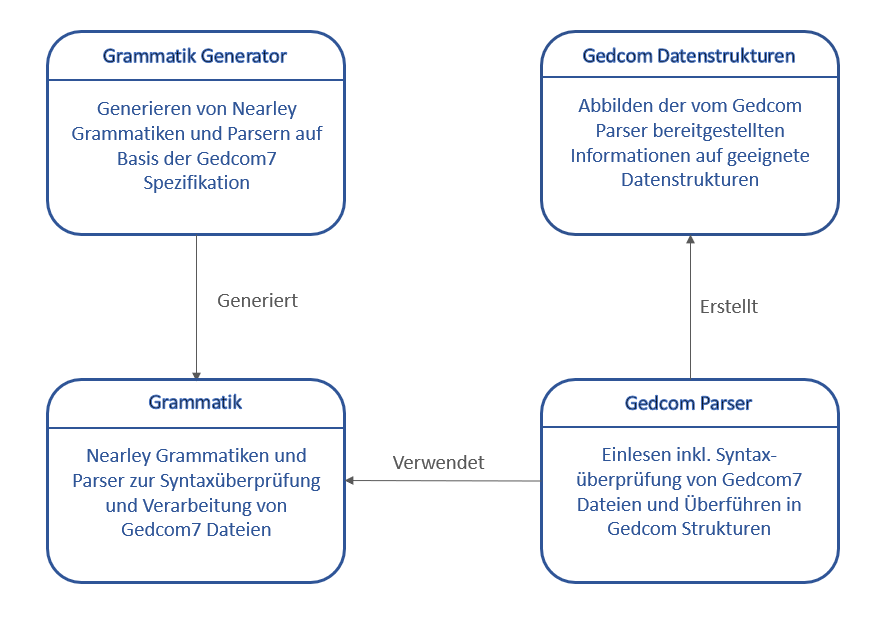
\includegraphics[width=0.85\textwidth]{images/konzept_allgemein.png}
	\caption{Allgemeiner Aufbau}
	\label{fig: Allgemeiner Aufbau}
\end{figure}

Die Bibliothek \textit{gedcom7.js} lässt sich wie in \hyperref[fig: Allgemeiner Aufbau]{Abbildung 4.1} dargestellt in vier logische Teile gliedern. Das zentrale Element ist der \textsc{Gedcom Parser}, mit dem Dateien oder Strings im in Abschnitt \ref{sec: GEDCOM Version 7} vorgestellten Format \textit{Gedcom7} eingelesen werden und mit Hilfe von \hyperref[sec: Nearley]{\textit{Nearley}} auf Korrektheit der Syntax überprüft werden können. Die dafür zugrundeliegende Grammatik wird mit Hilfe eines \textit{Grammatik Generators} generiert, der die in \cite{GEDCOM} definierte Spezifikation in eine Nearley-konforme Syntax überführt. Die so eingelesenen Informationen werden in Gedcom Datenstrukturen gespeichert, die verändert und erweitert werden und anschließend im Format Gedcom7 ausgegeben werden können. In den folgenden Abschnitten werden die vier Teile und das Zusammenspiel dieser in detaillierter Form vorgestellt.

%========================================================================================
% SECTION: GEDCOM GRAMMATIK
%========================================================================================
\section{Gedcom Grammatik}
\label{sec: Konzept - Gedcom Grammatik}
Eine wichtige Anforderung an die Bibliothek \textit{gedcom7.js} ist, dass die Syntax von Dateien oder Strings, die eingelesen werden, gemäß der Gedcom7-Spezifikation überprüfbar sein soll. Da die Gedcom Datenstrukturen veränderbar und erweiterbar sein sollen, ist es wichtig, dass eine Syntaxüberprüfung nach Änderungen auf einfache Weise möglich ist. Umgesetzt wird diese Syntaxüberprüfung mit Hilfe des in \hyperref[sec: Nearley]{Kapitel 2.3} vorgestellten JavaScript-Parser-Toolkits \textit{Nearley}. Mit \textit{Nearley} können auf einfach Weise, menschenlesbare Grammatiken erstellt und zu einem \textit{Nearley-Parser} kompiliert werden. Von großem Vorteil ist dabei, dass Features wie Postprozessoren und die Implementierung eines Lexers unterstützt werden. 

\subsection{Pre- und Postprozessor}
\label{subsec: Konzept - Gedcom Grammatik - Pre- und Postprozessor}
Standardmäßig gibt ein \textit{Nearley-Parser} jedes Zeichen, das mit einer Regel überein-\\stimmt, als Array zurück \cite{NearleyDoc}. Bei komplexeren Grammatiken wie der Gedcom7 Spezifikation führt dies dazu, dass sehr viele Arrays ineinander verschachtelt werden, sodass schnell zweistellige Verschatlungsgrade erreicht werden, was ein Weiterarbeiten mit den Ergebnissen erschwert. Mit Hilfe von Postprozessoren können jeder \textit{Nearley Regel} Verarbeitungsanweisungen zugewiesen werden, sodass die Ergebnisse beispielsweise im JSON-Format zurückgegeben werden. Auf diese Weise können die eingelesenen Dateien bereits bei der Syntaxüberprüfung in eine passende Darstellungsform gebracht werden, sodass eine leichte Überführung in die passende Gedcom Datenstruktur möglich ist.

Desweiteren kann ein Lexer verwendet werden, um die Arbeit mit \textit{Nearley} zu optimieren. Ein \textit{Nearley-Parser} teilt die Eingabedaten standardmäßig in einen Strom von einzelnen Zeichen, die sequentiell abgearbeitet werden, was auch als \textit{Scannerless Parsing} bezeichnet wird \cite{NearleyDoc}. Ein Lexer ist eine Art Preprozessor, der die Eingabedaten in größere Einheiten, die sog. \textit{Tokens} zusammenfasst \cite{NearleyDoc}. Auf diese Weise wird der Aufwand beim Parsen verringert und die Interpretation der Eingabedaten fällt oft leichter. Ein einfaches Beispiel hierfür ist eine Regel die einen Zahlenwert erwartet. Ist der Eingabewert beispielsweise "137", würde ein \textit{Nearley-Parser} standardmäßig jede Ziffer einzeln einlesen und im Postprozessor müsste definiert werden, dass die aufeinanderfolgenden Ziffern als ein Zahlenwert interpretiert werden sollen. Mit Hilfe eines Lexers könnte eine einfache Regel definiert werden, die den kompletten Zahlenwert als ein Token vorverarbeitet. Im Rahmen dieser Arbeit wurde der JavaScript Lexer \textit{Moo.js} \cite{MooDoc} verwendet. \textit{Moo.js} zeichnet sich durch seine Geschwindigkeit aus und wird von \textit{Nearley} als Lexer unterstützt.\footnote{Laut den Entwicklern ist Moo.js der schnellste JavaScript-Lexer und $\sim$2-10 mal schneller als herkömmliche Lexer \cite{MooDoc}.} 
\newpage
\subsection{Nearley-Parser für Gedcom7}
\label{subsec: Konzept - Gedcom Grammatik - Nearley-Parser für Gedcom7}
Da sowohl die Gedcom7- als auch die Nearley Syntax auf \hyperref[sec: Nearley]{EBNF-Sprachkonzepten} basieren, lässt sich die Gedcom7 Spezifikation ohne weiteres in eine Nearley Grammatik übersetzten, die dann zu einem Nearley-Parser kompiliert werden kann. Wird diesem Nearley-Parser eine Gedcom7-Datei (.ged) kodiert als UTF-8 Zeichenkette übergeben, erfüllt dieser die folgenden zwei Aufgaben:

\vspace{1em}
\textbf{1. Überprüfung der Gedcom7 Syntax} \vspace{0.35em} \\
Der Nearley-Parser überprüft den übergebenen Gedcom7-String Line für Line, indem er alle Zeichen (bzw. Tokens) sequentiell liest, bis ein End-Of-Line (EOL) Token  gefunden wird. Nach jedem Zeichen das eingelesen wird, überprüft der Parser, welche in der Grammatik definierten Regeln durch das neu eingelesene Zeichen nicht mehr mit der Zeichenkette übereinstimmen und verwirft diese. Wird ein EOL Token gelesen werden die Postprozessoren aller übereinstimmenden Regeln ausgeführt und ein Array mit den Ergebnissen dieser Postprozessoraufrufe als Ergebnis der Line zurückgegeben. Da die Gedcom7 Grammatik nicht mehrdeutig ist, findet der Parser bei korrekter Gedcom7 Syntax immer ein eindeutiges Ergebnis (d.h. beim Erreichen des EOL Tokens ist maximal eine übereinstimmende Regel übrig). Werden bei diesem Prozess alle Regeln der Grammatik ausgeschlossen, bevor ein EOL Token gelesen wird, ist die Syntax des übergebenen Gedcom7-Strings nicht korrekt und das Parsen wird mit einem Syntaxfehler abgebrochen. Da die Zeichenkette sequentiell abgearbeitet wird, kann bei auftretendem Fehler genau aufgezeigt werden, welche Line und welches Zeichen fehlerhaft sind.

\vspace{1em}
\textbf{2. Extrahieren der Structure-Informationen} \vspace{0.35em} \\
Eine weitere Aufgabe des Nearley-Parsers ist es, die Structure-Informationen des Gedcom7-Strings zu extrahieren, sodass im nächsten Schritt eine einfache Über-führung in entsprechende Gedcom Datenstrukturen möglich ist. Durch den sequentiellen Aufbau einer Gedcom7 Datei wird eine Structure immer vor ihren Substructures definiert. Da das erste Token jeder Line stets das Level der Line repräsentiert, kann der Nearley-Parser die Abhängigkeiten der Lines zueinander zuordnen und es ist zu jedem Zeitpunkt eindeutig, welcher Superstructure eine Structure zugeordnet werden soll. Folgende Informationen können also durch den Nearley-Parser extrahiert werden: 
\begin{itemize}
	\item \textbf{Inhalt der Line}: Die in Abschnitt \ref{sec: GEDCOM Version 7} vorgestellten Bestandteile einer Line können ausgelesen und zugeordnet werden.
	\item \textbf{Datentyp}: Sofern ein Payload in der Line vorhanden ist, kann mit Hilfe der URI der Datentyp des Payloads bestimmt werden
	\item \textbf{Superstructure}: Zu jeder Line kann die entsprechende Superstructure angegeben werden, sofern es sich nicht um einen Record (Structure mit Level 0) handelt, die keine Superstructure besitzen
	\item \textbf{Substructures}: Hat eine Sturktur eine oder mehrere Substructures, können diese auf Basis des Levels der Lines bestimmt werden
\end{itemize}

%========================================================================================
% SECTION: GRAMMATIK GENERATOR
%========================================================================================
\section{Grammatik Generator}
\label{sec: Konzept - Grammatik Generator}
% Warum Grammatik Generator -> Anforderung erweiterbar
% Wie umgesetzt? -> JS-Definitionsdateien einlesen 
% Ablauf -> einlesen, grammatik erstellen, kompilieren,
In der Gedcom7 Spezifikation werden 181 Structuretypes verteilt auf 7 Records definiert, die alle in einer Line der Form
\begin{lstlisting}[frame=none]
	Level  D  [Xref  D]  Tag  [D  LineVal]  EOL
\end{lstlisting}
dargestellt werden. Sollen diese Structuretypes in eine Nearley Grammatik überführt werden, muss für jede dieser Structures und jede mögliche Kombination an Substructures eine Regel erstellt werden. Da dies eine sehr repetitive Aufgabe ist und sich die Regeln nur an bestimmten Stellen unterscheiden, lässt sich die Grammatikerstellung durch einen Grammatik Generator automatisieren. Dazu können Definitionsdateien erstellt werden, die die für alle Structuretypes die folgenden Informationen bereithalten: 
\begin{itemize}
	\item \textbf{URI}: Die URI des Structuretypes wird benötigt, um eine Structure eindeutig zuordnen zu können 
	\item \textbf{LineType}: Der LineType gibt an, wie die Line aufgebaut ist - also ob bspw. ein Cross-Reference-Identifier oder ein Payload vorhanden sind
	\item \textbf{Datatype}: Sofern ein Payload in der Line vorhanden ist, kann über den Datatype die Syntax des Payloads ermittelt werden
	\item \textbf{Tag}: Der Tag wird benötigt, um die Line einer Nearley Regeln zuordnen zu können
	\item \textbf{Substructures}: In der Gedcom7 Spezifikation sind für alle Structuretypes alle zulässigen Substructures definiert. Mit dieser Information können alle syntaktisch korrekten Structures in Nearley Regeln abgebildet werden.
	\item \textbf{Level}: Um eine eindeutige Grammatik zu generieren, müssen die Level mit denen ein jeweiliger Structuretype auftreten kann, zwingend mit angegeben werden. Da in der Gedcom7 Spezifikation Tags mehrfach für verschiedene Structuretypes verwendet werden, kann nicht einfach ein generisches Level für die Regeln verwendet werden, das ganzzahlige Werte akzeptiert, da die entstehende Grammatik damit mehrdeutig wäre. Ein Beispiel hierfür sind die Structures \textit{g7:HEAD-DATE} und \textit{g7:DATE-exact} im Gedcom Header. Mit einem generischen Level wären die Regeln für beide Structuretypes identisch mit 
	\begin{lstlisting}[frame=none]
	  Level  D  "DATE"  D  DateExact  EOL
	\end{lstlisting}
	Wird eine solche Line als Substructure eines Header Records von dem Nearley Parser gelesen, kann dieser nicht entscheiden, ob es sich um ein \textit{g7:HEAD-DATE} oder ein \textit{g7:DATE-exact} handelt und würde somit zwei Ergebnisse aufrecht erhalten. Um diese Mehrdeutigkeit zu verhindern, wird das Level in der Definition angegeben. Da die Structure \textit{g7:HEAD-DATE} mit dem Level $+1$ und \textit{g7:DATE-exact} mit Level $+3$ bezogen auf den zugrundeliegenden Header Record vorliegen, können die Lines vom Parser eindeutig unterschieden werden.
\end{itemize}
\newpage
Anhand dieser Informationen kann der Grammatik Generator automatisiert Nearley Regeln formulieren. Diese Regeln können zu einer Grammatik zusammengefasst und anschließend vom Generator zu einem Nearley-Parser kompiliert werden. Anhand des LineTypes kann der Generator den Regeln die passenden Postprozessoren zuweisen, die für das Extrahieren der Structure Informationen zuständig sind. Auf diese Weise kann ein voll funktionaler Nearley-Parser automatisiert generiert werden, der die Gedcom7-Syntax vollständig parsen und alle für die weitere Verarbeitung benötigten Informationen extrahieren kann. 


Ein weiterer großer Vorteil an dieser Automatisierung ist, dass zur Erfüllung der Anforderung der einfachen Erweiterbarkeit der Bibliothek beigetragen wird. Sollte die Grammatik in zukünftigen Projekten erweitert werden, bspw. wenn in einer neuen Version des Gedcom Standards weitere Structuretypes definiert werden, ist dies auf einfache und verständliche Weise durch das Hinzufügen neuer Einträge in die Definitionsdatei des Grammatik Generators möglich. 


Desweiteren bildet der Grammatik Generator ein Fundament für einen wichtigen Use-Case, der in weiterführenden Arbeiten adressiert werden sollte: der Möglichkeit Extensions zu definieren. Die Gedcom7 Spezifikation definiert die wichtigsten Strukturen zur Speicherung genealogischer Informationen - für alle Informationen, die über diese Standardstrukturen hinausgehen, müssen Extensions definiert werden. Da genealogische Informationen sehr vielfältig sein können, sind Extensions ein probates Mittel, dass in vielen Anwendungen genutzt wird. Mit Hilfe des Grammatik Generators kann die Definition von Extensions umgesetzt werden, indem eine Schnittstelle zum Generator entwickelt wird, die dem Benutzer zur Verfügung gestellt wird. Über diese Schnittstelle kann die Definitionsdatei erweitert und anschließend die Grammatik neu generiert und kompiliert werden. Auf diese Weise könnte die Bibliothek auf die Anforderung aller Benutzer angepasst werden. 
%========================================================================================
% SECTION: GEDCOM STRUKTUREN
%========================================================================================
\section{Gedcom Datentrukturen}
\label{sec: Konzept - Gedcom Strukturen}
Die zentrale Struktur in einer Gedcom7 Datei ist das sog. \textit{Dataset}. Jedes Dataset muss mit einer \textit{Header-Structure} beginnen, der Metadaten über das gesamte Dataset beinhaltet und dabei u.a. Aussagen über den Ort und Zeitpunkt der Erstellung und den Ersteller des Datasets selbst machen kann. Die Mindestanforderung an den Header ist, dass die verwendete Gedcom Version in einer dafür vorgesehenen Structure spezifiziert ist. Abgeschlossen wird jedes Dataset mit einer \textit{Trailer Line}, die das Ende des Datasets repräsentiert. Eine minimales Gedcom7 Dataset sieht also wie folgt aus:
\newpage
{
\begin{lstlisting}
	0 HEAD
	1 GEDC
	2 VERS 7.0
	0 TRLR
\end{lstlisting}
\captionof{lstlisting}{Minimales Gedcom7 Dataset}
\label{lst: minimales dataset}
}
\vspace{1em}
Alle genealogischen Informationen können in einem oder mehreren Records festgehalten werden. Folgende Records sind in der Gedcom7 Spezifikation definiert:
\begin{itemize}
	\label{liste records}
	\item \textbf{Family (FAM)}: Der Family Record wurde ursprünglich so strukturiert, dass er eine Familie mit einem männlichen Ehemann und einer weiblichen Ehefrau repräsentiert. Um die Migration von bestehenden Gedcom-Dateien auf Gedcom7 zu erleichtern, wurde die Benamung der Strukturen beibehalten. Trotzdem sollen in Gedcom7 Familien, Heirat, Zusammenleben und Adoption unabhängig vom Geschlecht der Partner angegeben werden können und daher das Geschlecht und die Rollen von Partnern nicht aus der Husband- bzw. Wife Struktur abgeleitet werden.
	\item \textbf{Individual (INDI)}: Zusammenstellung von Fakten und Hypothesen über eine Person. Diese können aus verschiedenen Quellen stammen, die durch Quellenangaben dokumentiert werden können.
	\item \textbf{Multimedia (OBJE)}: Eine Referenz zu einer oder mehrerer digitaler Dateien, angereichert mit Informationen über den Inhalt und den Typ der Datei.
	\item \textbf{Repository (REPO)}: Beinhaltet Informationen über Personen oder Institutionen, die eine Sammlung von Quellen besitzen.
	\item \textbf{Shared Note (SNOTE)}: Eine Sammlung von Informationen, die nicht vollständig in andere Strukturen passen. Beispiele wären Forschungsnotizen, alternative Interpretationen oder Argumentationen
	\item \textbf{Source (SOUR)}: Beschreibt eine Quelle, indem auf bestimmte Dokumente oder Verzeichnisse verwiesen wird.
	\item \textbf{Submitter (SUBM)}: Beschreibt eine Person oder eine Institution, die im Dataset enthaltene Informationen beigesteuert hat.
\end{itemize}
In der Gedcom7 Spezifikation ist festgelegt, welche Structures Teil eines bestimmten Records sein dürfen. Beispielsweise darf eine \textit{HUSB}-Structure nur in einem Family Record vorliegen - ein \textit{CREATION\_DATE} dahingegen kann für alle Records definiert werden. Alle Lines, die in einem Gedcom7 Dataset vorliegen sind Structures, die über Super- und Substructures zueinander ins Verhältnis gesetzt werden. Auch ein Record ist eine Structure, jedoch mit der Besonderheit, dass ein Record im Gegensatz zu allen anderen Structures keine Superstructure besitzt. Die genauen Verhältnisse dieser Datenstrukturen ist in Abbildung \ref{fig: Gedcom Strukturen} dargestellt. Im folgenden werden die Datenstrukturen, mit denen eine Gedcom7 Datei in der Bibliothek \textit{gedcom7.js} abgebildet wird, vorgestellt.
\newpage
\subsection{Structure}
\label{subsec: Konzept - Gedcom Strukturen - Structure}
In der Bibliothek \textit{gedcom7.js} wird jede Line, die vom Parser gelesen wird, in Form einer Structure abgebildet (siehe Abbildung \ref{fig: Gedcom Strukturen}). Diese Datenstruktur hält alle Informationen wie Level, Tag und LineValue der Line bereit und enthält zudem Verweise auf die Superstructure und alle Substructures. Eine wichtige Anforderung ist zudem, dass die eingelesene Gedcom7 Datei veränderbar und erweiterbar sein soll. Daher enthält die \textit{Structure} Datenstruktur Methoden mit der Substructures hinzugefügt bzw. entfernt werden können und mit denen der Payload der Structure verändert werden kann. Um die veränderte Datenstruktur als Gedcom7 Datei speichern zu können, muss jede Structure als Gedcom7 konforme Line ausgegeben werden können. Außerdem werden zwei spezielle Structures definiert, die \textit{Datatype Structures} und \textit{Records}.

\vspace{1em}
\textbf{1. Records} \vspace{0.5em} \\
Die in der Einleitung dieses Kapitels aufgeführten \hyperref[liste records]{Records}, wie z.B. der Family Record, sind die Superstructures aller weiteren Structuretypes und haben somit besondere Anforderungen. Daher werden in \textit{gedcom7.js} alle Records in Form einer eigenen Record Datenstruktur abgebildet, die \textit{Structure} erweitert. Dabei sollen Methoden bereitgestellt werden, mit denen die Informationen, die in den Substructures enthalten sind, extrahiert werden können. Ein Beispiel hierfür wäre eine Methode, die alle Informationen über die Residenz einer Familie, die über viele Substructures verteilt sind, zusammenfasst und in übersichtlichem Format zurückgibt. In einem Gedcom7 Record kann zudem über eine \textit{Restriction Structure} der Zugriff auf Informationen dieses Records eingeschränkt werden. Die Record Datenstruktur sollte diese Einschränkungen verwalten und die Ausgabe von Informationen dementsprechend anpassen. Außerdem sollen alle Records Möglichkeiten zur Syntaxüberprüfung des Records und all seiner Substructures besitzen, sodass nach dem Hinzufügen einer Structure in einen Record, die Syntax des Records überprüft werden kann, um zu entscheiden, ob das Hinzufügen syntaktisch korrekt war. Dies bietet den Vorteil, dass nicht jedes Mal die Syntax des gesamten Datasets überprüft werden muss, obwohl sich nur ein Record verändert hat.

\vspace{1em}
\textbf{2. Datatype Structures} \vspace{0.5em} \\
Der Payload von Lines kann verschiedene Datentypen haben, die in der Gedcom7 Datei als Zeichenkette kodiert sind. Handelt es sich dabei um einen einfachen LineValue vom Datentyp \textit{Text} ist es ausreichend, diesen als Zeichenkette in der Structure zu hinterlegen. Bei komplexeren Datentypen wie \textit{Date} ist es jedoch notwendig, die Structure um Methoden und Eigenschaften zu erweitern, die die weitere Verarbeitung erleichtern. Daher werden für komplexere Datentypen wie \textit{Date} oder \textit{Personal Name} spezielle \textit{Datatype Structures} bereitgestellt, mit denen beispielsweise das Datum eines Events in ein JavaScript konformes Date-Objekt überführt werden kann.

\begin{figure}[h]
	\centering
	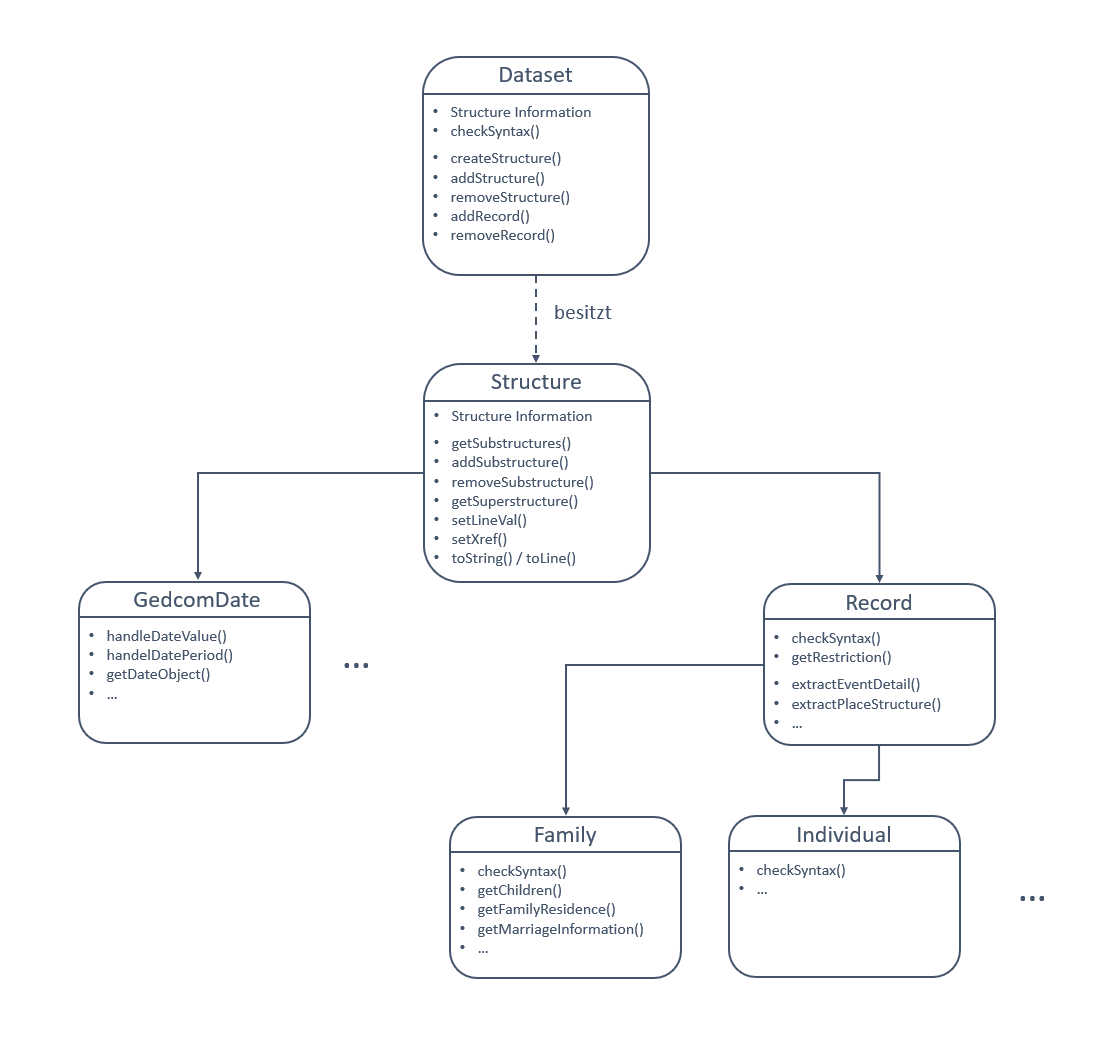
\includegraphics[width=1.0\textwidth]{images/konzept_structure.png}
	\caption{Gedcom Strukturen}
	\label{fig: Gedcom Strukturen}
\end{figure}

\subsection{Dataset}
\label{subsec: Konzept - Gedcom Strukturen - Dataset}
Die in Abschnitt \ref{subsec: Konzept - Gedcom Strukturen - Structure} beschriebenen Structures werden in einer \textit{Dataset} Datenstruktur zusammengefasst, die alle genealogischen Informationen einer Gedcom7 Datei enthält. Die Hauptaufgabe des Datasets besteht darin, Structures zu erstellen und zu verwalten. Wird eine Gedcom7 Datei mit korrekter Syntax mit dem in \ref{subsec: Konzept - Gedcom Grammatik - Nearley-Parser für Gedcom7} vorgestellten Nearley Parser eingelesen, extrahiert dieser alle Structure Informationen. Anschließend kann ein \textit{Dataset} erstellt werden, das all diese Informationen einliest, daraus Structures erstellt und die Zusammenhänge zwischen diesen Structures modelliert, sodass, eine Art Baumstruktur mit allen Records entsteht. Um ein Dataset mit neuen genealogischen Informationen anzureichern, sollen Methoden zum Hinzufügen bzw. zum Entfernen von Records bereitgestellt werden. Da das Hinzufügen bzw. Entfernen von Strukturen zu einer inkorrekten Gedcom7 Syntax führen kann, müssen Methoden zur Syntaxüberprüfung implementiert werden. Des Weiteren stellt das Dataset Metainformationen über eine Gedcom7 Datei zur Verfügung und sollte bestimmte Anforderungen überprüfen, die in der Gedcom7 Spezifikation angegeben werden. Beispiele hierfür sind, dass jede Gedcom7 Datei mit dem \textit{Byte-Order-Mark} beginnen sollte oder dass alle Structure, auf die über einen Cross-Reference-Identifier verwiesen wird, definiert seien müssen, bevor auf diese verwiesen wird. 
%========================================================================================
% SECTION: GEDCOM PARSER
%========================================================================================
\section{Gedcom Parser}
Die in diesem Kapitel vorgestellten Konzepte und Datenstrukturen werden alle im \textsc{Gedcom Parser} vereinigt, der die zentrale Instanz der Bibliothek \textit{gedcom7.js} darstellt. Abbildung \ref{fig: Sequenz Gedcom Parser} zeigt ein Sequenzdiagramm, das den allgemeinen Ablauf beim Einlesen einer Gedcom7 Datei mit dem \textsc{Gedcom Parser} zeigt.\\ 
Der \textsc{Gedcom Parser} ließt eine Gedcom7 Datei ein und konvertiert diese in eine Zeichenkette. Die Zeichenkette kann dann an einen Nearley Parser übergeben werden, der diese Line für Line ließt, die Syntax überprüft und dabei die Structure Informationen extrahiert. Ist die Syntax der Gedcom7 Datei korrekt, werden die gesammelten Structure Informationen an den Gedcom Parser zurückgegeben - anderenfalls wird das Einlesen mit einer Fehlermeldung beendet. Anschließend überprüft der Gedcom Parser die Kardinalität der eingelesenen Structures (beispielsweise darf nur eine \textit{HUSB}-Struktur pro Family Record enthalten sein).\footnote{Die Kardinalitätsüberprüfung wurde in den Gedcom Parser ausgelagert, da Nearley ein Streaming-Parser ist und somit zu keinem Zeitpunkt weiß, ob noch weitere Eingaben zu erwarten sind. Daher werden Konzepte wie Kardinalitätsüberprüfungen nicht von Nearley unterstützt. \cite{NearleyDoc}}. Sofern keine Fehler bei der Kardinalitätsüberprüfung gefunden werden, wird ein neues Dataset erstellt und die von Nearley extrahierten Structure Informationen an das Dataset übergeben. 


Das Dataset generiert den Header und den Trailer, der in jedem Dataset vorhanden sein muss und erstellt anschließend alle Structures auf Basis der Structure Informationen. Dazu wird jeder Eintrag der Structure Informationen auf den Structure Type untersucht (Record, Datatype Structure oder allgemeine Structure) und auf Basis dessen eine Structure mit allen Informationen erstellt. Diese Structure wird dann in das Dataset eingegliedert, indem die entsprechende Superstructure und alle Substructures zugewiesen werden. Sind alle Structures erstellt, wird überprüft, ob dass alle Cross-Reference-Identifier, auf die im Dataset verwiesen wird auch innerhalb des Datasets definiert sind. Ist dies der Fall, wird das Dataset zurückgegeben. Dieses Dataset kann dann wie in Abschnitt \ref{sec: Konzept - Gedcom Strukturen} beschrieben verändert und erweitert werden.

\begin{figure}[h]
	\centering
	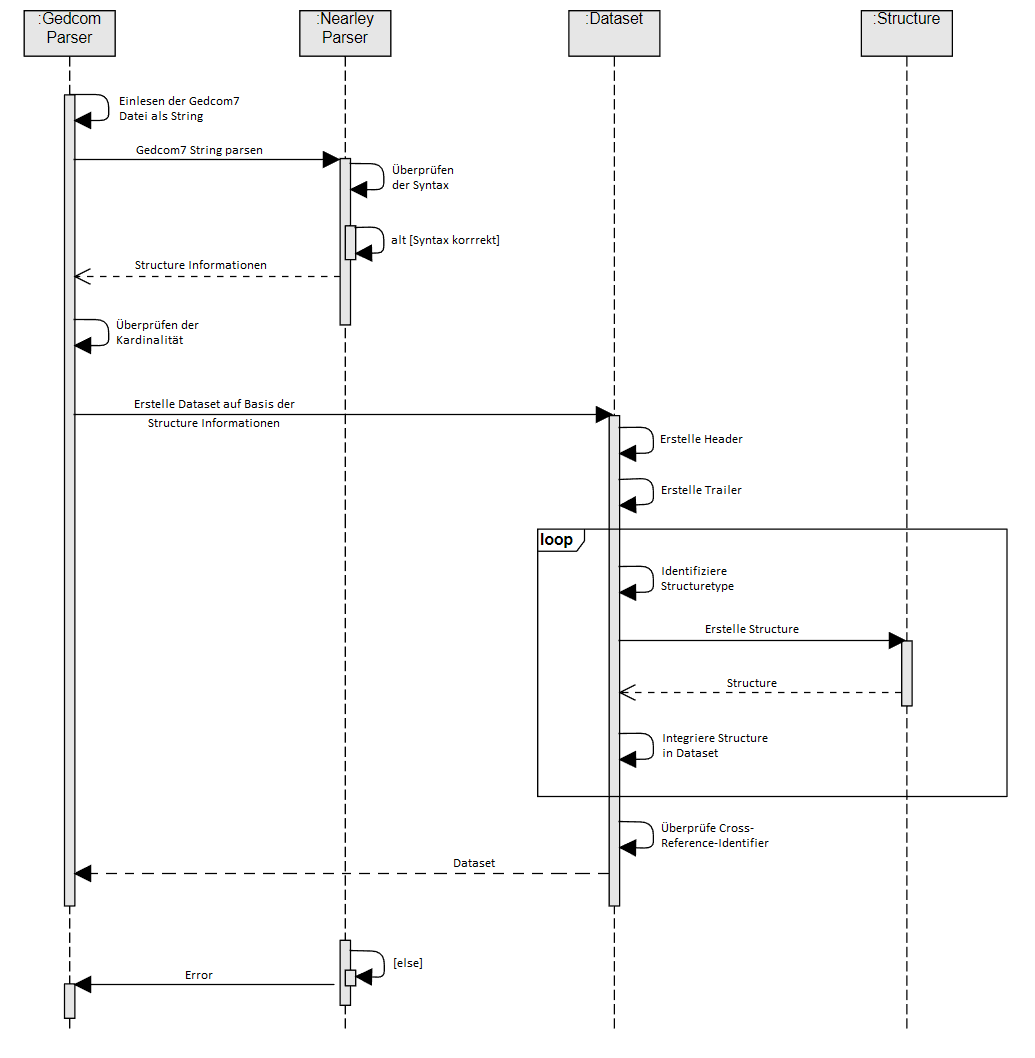
\includegraphics[width=1\textwidth]{images/konzept_sequenz.png}
	\caption{Ablauf Gedcom Parser}
	\label{fig: Sequenz Gedcom Parser}
\end{figure}
\label{sec: Konzept - Gedcom Parser}

\chapter{Implementierung \& Test}
\label{chap: Implementierung und Test}
In diesem Kapitel wird beschrieben wie das im Kapitel \ref{chap: Konzept} vorgestellte Konzept in der Bibliothek \textit{gedcom7.js} implementiert wird. Dazu wird zuerst darauf eingegangen, wie die Gedcom7 Spezifikation in der Nearley Grammatik abgebildet wird und wie diese Grammatikerstellung automatisiert werden kann. Anschließend wird dargestellt, wie die in Abschnitt \ref{sec: Konzept - Gedcom Strukturen} vorgestellten Gedcom Datenstrukturen implementiert wurden. Es wird gezeigt, wie diese Komponenten im \textsc{Gedcom Parser} vereinigt werden und in einem detailierten Beispiel wird die Verwendung des Parsers demonstriert. Zum Schluss wird darauf eingegangen, wie die Bibliothek und die darin enthalten Funktionen getestet wurden.

%========================================================================================
% SECTION: GEDCOM GRAMMATIK
%========================================================================================
\section{Gedcom Grammatik}
\label{sec: Implementierung - Gedcom Grammatik}
Da die Gedcom7- sowie die Nearley Syntax beide auf EBNF-Sprachkonzepten basieren, lässt sich die Gedcom7 Spezifikation ohne weiteres in eine Nearley Grammatik übersetzten. Im folgenden wird gezeigt, wie die Grammatik erstellt wurde und welche Postprozessoren verwendet wurden. 
\subsection{Gedcom7 Syntax in Nearley}
\label{subsec: Implementierung - Gedcom Grammatik - Gedcom7 Syntax in Nearley}
Um Nearley Regeln für eine Gedcom Line zu definieren, können die folgenden Tokens für das Leerzeichen, den \textit{Cross-Reference Identifier} und die End-Of-Line Zeichenfolge in Form von regulären Ausdrücken definiert werden.
\vspace{1em}
\begin{javascript}{Tokens für eine Gedcom Line, definiert als regulärer Ausdruck}{lst: tokens gedcom line}
	D    : /[ ]/
	Xref : /\@[A-Z0-9\_]+\@/	
	EOL  : /(?:\r\n?|\n)/
\end{javascript}
\newpage
{
\noindent
Diese regulären Ausdrücke werden in der Vorverarbeitungsphase vom Moo-Lexer verwendet, um zusammenhängende Zeichen zu Tokens zu gruppieren, die dann in der Nearley Grammatik über den Tokennamen mit einem vorangestellten \%-Zeichen angesprochen werden können. Soll nun die erste Line eines Family-Records geparsed werden, könnte dies mit der folgenden Nearley-Regel umgesetzt werden.
}
\vspace{0em}
\begin{javascript}{Nearley Regel zum parsen eines Family Records}{lst: nearley regel family record first line}
	record_FAM -> "0"  %D  %Xref  %D  "FAM"  %EOL 
\end{javascript}
\vspace{1em}
Diese Regel akzeptiert eine Line mit dem Level 0, einem syntaktisch korrekten Cross-Reference-Identifier, dem Tag \textit{FAM} gefolgt von einem EOL-Token. Getrennt werden die Bestandteile durch ein Leerzeichen. Sollen nun ebenfalls HUSB- und WIFE Structures als Substructures des Family Records akzeptiert werden, könnte die Nearley Grammatik wie folgt erweitert werden.
\vspace{1em}
\begin{javascript}{Nearley Regel zum parsen eines Family Records mit HUSB- und WIFE Substructures}{lst: nearley regel family record with husb and wife}
	record_FAM
		-> "0"  %D  %Xref  %D  "FAM"  %EOL 
		|  record_FAM  record_FAM_Substructs:+
	
	record_FAM_Substructs 
		-> "1"  %D  "HUSB"  %D  %Xref  %EOL
		|  "1"  %D  "WIFE"  %D  %Xref  %EOL 
\end{javascript}
\vspace{1em}
Auf diese Weise nimmt würde der Nearley Parser einen Family Record ohne Substructures und einen Family Record mit beliebig vielen HUSB- und WIFE Structures als Substructures als Eingabe akzeptieren. Für die HUSB- und WIFE Structure ist als Payload ein Cross-Reference-Identifier angegeben, da in diesen Structures auf ein \textit{Individual} Record verwiesen wird.

Sollen nun die weiteren Lines aus Listing \ref{lst: family record example} ebenfalls in die Grammatik aufgenommen werden, müssen Regeln für die Datentypen der Payloads des MARR-Events und der NCHI-Structure definiert werden. Die Anzahl der Kinder wird als  \textit{Integer} Datentyp kodiert, also ein Folge von Dezimalziffern. Nach der Gedcom7 Spezifikation dürfen \textit{Integer} Werte nicht leer sein und führende Nullen sind erlaubt, sollten aber vermieden werden. Eine Regel für den Datentyp \textit{Integer} kann also wie in Listing \ref{lst: nearley regel integer} dargestellt, formuliert werden.
\vspace{1em}
\begin{javascript}{Nearley Regel für den Datentyp \textit{Integer}}{lst: nearley regel integer}
	digit    ->  [0-9]
	Integer  ->  digit:+
\end{javascript}
\vspace{1em}
Für das \textit{MARR}-Event, also die Hochzeit der Ehepartner der Familie, ist eine\\\textit{DATE}-Structure zur Spezifikation des Datums der Hochzeit hinterlegt. Dieses Datum wird mit dem Datentyp \textit{DateValue} kodiert, der im Gegensatz zum \textit{Integer} wesentlich mehr Regeln umfasst. Ein \textit{DateValue} kann auf vier verschiedene Weisen dargestellt werden:
\begin{enumerate}
	\item \textit{date}: ``JULIAN 13 MAR 1998 BCE''\\Ein mehr oder weniger genau spezifiziertes Datum
	\item \textit{datePeriod}: ``FROM 15 FEB 2001 TO 23 MAR 2001''\\Ein Zeitintervall, dass von einem Startdatum bis zu einem Enddatum angegeben wird
	\item \textit{dateRange}: ``BET 15 FEB 2001 AND 23 MAR 2001''\\Ein ungenaueres Zeitintervall, bei dem nur Grenzen angegeben werden
	\item \textit{dateApprox}: ``ABT 15 FEB 2001''\\Eine Schätzung des Datums (ABT $x$: genaues Datum unbekannt, aber nahe $x$)
\end{enumerate}
Diese Zusammenhänge ergeben die in Listing \ref{lst: nearley regel date} dargestellten Nearley Regeln für die Definition des Datentyps \textit{DateValue}.
\vspace{1em}
\begin{javascript}{Nearley Regel für den Datentyp \textit{DateValue}}{lst: nearley regel date}
	DateValue   ->  (date | DatePeriod | dateRange | dateApprox):?
		
	date		->  (calendar  D):?  
					((day  D):?  month  D):?  
					year  
					(D  epoch):?
	datePeriod  ->  ("FROM"  D  date  D):?  "TO"  D  date
	dateApprox  ->  ("ABT" | "CAL" | "EST")  D  date 
	dateRange   ->  "BET"  D  date  D  "AND"  D  date  
					|   "AFT"  D  date  
					|   "BEF"  D  date 
	
	calendar 	->  "GREGORIAN" | "JULIAN" | "FRENCH_R" | "HEBREW"
	day      	->  Integer  
	year 	 	->  Integer
	month    	->  Tag
	epoch    	->  "BCE" | Tag
	Tag 		->  upperCaseLetter  |  digit  |  underscore 
\end{javascript}
\vspace{1em}
Werden all diese Regeln zusammengefasst lässt sich eine Grammatik definieren, die den Family Record aus Listing \ref{lst: family record example} als Eingabe akzeptiert. Diese Grammatik ist in Listing \ref{lst: vollständige nearley grammatik family record} dargestellt.

Mit diesem Vorgehen können Nearley Regeln für alle Datentypen, Structures und Records definiert werden, die zu einer Grammatik für die Syntaxüberprüfung von Gedcom7 Dateinen zusammengesetzt werden können.
\vspace{1em}
\begin{javascript}{Nearley Grammatik für den Family Record aus Listing \ref{lst: family record example}}{lst: vollständige nearley grammatik family record}
	record_FAM_Substructs
		-> "0"  %D  %Xref  %D  "FAM"  %EOL 
		|  record_FAM  record_FAM_Substructs:+
		
	record_FAM_Substructs 
		-> "1"  %D  "HUSB"  %D  %Xref  %EOL
		|  "1"  %D  "WIFE"  %D  %Xref  %EOL 
		|  "1"  %D  "NCHI"  %D  Integer  %EOL 
		|  structure_MARR 
		
	structure_MARR
		-> "1"  %D  "MARR" %EOL
		|  structure_MARR  
		
	structure_DATE
		-> "2" %D  "DATE"  %D  DateValue  %EOL
\end{javascript}
\vspace{1em}

\subsection{Nearley Postprozessoren}
\label{subsec: Implementierung - Gedcom Grammatik - Nearley Postprozessoren}
 Mit Hilfe von Postprozessoren können jeder Nearley Regel Verarbeitungsanweisungen zugewiesen werden. Für die Bibliothek \textit{gedcom7.js} werden die folgenden drei Nearley Postprozessoren implementiert.
\newpage
\textsc{\textbf{1. joinAndUnpackAll()}:} \vspace{0.5em} \\
Wie in Abschnitt \ref{subsec: Konzept - Gedcom Grammatik - Pre- und Postprozessor} beschrieben, überführt ein \textit{Nearley-Parser} jedes Zeichen, das mit einer Regel übereinstimmt, in ein Array. Bei komplexeren Grammatiken wie der Gedcom7 Spezifikation führt dies dazu, dass sehr viele Arrays innereinander verschachtelt werden, sodass schnell hohe Verschatlungsgrade erreicht werden. Ein Beispiel hierfür wäre der in Abschnitt \ref{subsec: Implementierung - Gedcom Grammatik - Gedcom7 Syntax in Nearley} definierte Datentyp \textit{DateValue}. Hier würde jeder Bestandteil eines DateValues in ein eigenes Array verschachtelt werden. Wird beispielsweise das Datum 
\begin{lstlisting}[frame=none]
			 	13 MAR 1998 BCE
\end{lstlisting}
ohne Postprozessoren verarbeitet, wird das Array
\begin{lstlisting}[frame=none]
		[13, , [MAR, , [1998, , [BCE, , ]]]]
\end{lstlisting}
zurückgegeben, dass eine Weiterverarbeitung sehr umständlich macht. Daher wird der Postprozessor \textit{joinAndUnpackAll()} implementiert, der über die JavaScript Funktion \textit{flat()} alle Elemente des Arrays rekursiv verkettet und anschließend über die Funktion \textit{join()} zu einer Zeichenkette zusammenfügt. Wird dieser Postprozessor einem Datentyp wie \textit{DateValue} zugewiesen, wird jedes syntaktisch korrekte Datum als Zeichenkette zurückgegeben und kann so direkt als LineValue für die weitere Verarbeitung verwendet werden. Die in Listing \ref{lst: nearley regel date} definierte Regel würde sich ergeben zu
\vspace{1em}
\begin{javascript}{Erweiterung der Nearley Regel für den Datentyp \textit{DateValue}}{lst: nearley regel date mit postprozessor}
	DateValue   
		->  (date | DatePeriod | dateRange | dateApprox):?
			 
\end{javascript}
\vspace{1em}

\textsc{\textbf{2. createStructure()}:} \vspace{0.5em} \\
Der Postprozessor \textit{createStructure()} wird verwendet, um die gelesene Line mit Structure Informationen anzureichern. In der Nearley Regel wird die Line selbst, der Typ und die in der Gedcom7 Spezifikation definierte URI der Line und die Structures bei denen eine Kardinalitätsüberprüfung notwendig ist an den Postprozessor übergeben. Für den in Listing \ref{lst: vollständige nearley grammatik family record} Family Record ergibt sich die Nearley Regel mit Postprozessoraufruf wie folgt:
\vspace{1em}
\begin{javascript}{Nearley Regel zum parsen eines Family Records mit Postprozessor}{lst: nearley regel family record mit postprozessor}
	record_FAM
		-> "0"  %D  %Xref  %D  "FAM"  %EOL
		 	
\end{javascript}
\vspace{1em}
Mit dem Parameter \textit{checkCardinalityOf} werden die URIs aller Structures angegeben, bei denen eine Kardinalitätsüberprüfung notwendig ist und ihnen wird die in der Gedcom7 Spezifikation definierte Kardinalität als Wert zugewiesen. Kardinalitätsüberprüfungen sind bei allen Substructures erforderlich, die für die Superstructure als notwendig definiert wurden (1:1 und 1:M) oder für die eine Maximale Anzahl festgelegt ist (also 0:1 und 1:1). In der Funktion \textit{createStructure()} werden alle Informationen abhängig vom übergebenen Type zusammengefasst und als JavaScript Objekt an den Parser zurückgegeben. Für einen Family Record ergibt sich die Funktion zu:
\vspace{1em}
\begin{javascript}{Postprocessor \textit{createStructure()} für einen Family Record}{lst: createStructure für Family Record}
	createStructure: (params) => {
		// create line object depending on type of line
		let lineObject = {};
		lineObject = { 
			level: line[0], 
			xref: line[2], 
			tag: line[4], 
			lineVal: '', 
			EOL: line[5] 
		};
		
		// return data object with structure information
		return {
			uri: params.uri,
			line: lineObject,
			type: params.type,
			lineValType: params.lineValType || null,
			superstructFound: false,
			substructs: [],
			checkCardinalityOf: params.checkCardinalityOf
		};
	}
\end{javascript}
\vspace{1em}

\textsc{\textbf{3. addSubstructure()}:} \vspace{0.5em} \\
Der Postprozessor \textit{addSubstructure()} wird verwendet, um die mit \textit{createStructure()} erstellten Structures miteinander zu verbinden und die Verhältnisse zwischen Superstructures und Substructures abzubilden. Im Falle des Family Records würde sich die in Listing \ref{lst: nearley regel family record mit postprozessor und substructs} dargestellte Regel ergeben. 
\vspace{1em}
\begin{javascript}{Vollständige Nearley Regel zum parsen eines Family Records mit Substructures}{lst: nearley regel family record mit postprozessor und substructs}
	record_FAM
		-> "0"  %D  %Xref  %D  "FAM"  %EOL
			
		
		|  record_FAM  record_FAM_Substructs:+
			
\end{javascript}
\vspace{1em}
Äquivalent zu Listing \ref{lst: nearley regel family record mit postprozessor} wird für die erste Line des Family Records der \textit{createStructure()} Postprocessor aufgerufen. Für alle Substructures die gefunden werden, wird ebenfalls der \textit{createStructure()} Postprocessor aufgerufen (die Regel für die Substructures ist aus Platzgründen nicht in Listing \ref{lst: nearley regel family record mit postprozessor und substructs} aufgeführt, kann aber äquivalent zu der Regel für den Family Record mit leicht veränderten Parametern definiert werden). Sind alle Substructures gefunden, wird der Postprozessor \textit{addSubstructure()} aufgerufen, der die Abhängigkeitsverhältnisse der Structures zueinander abbildet. Dazu werden beim Family Record alle gefundenen Subtructures in der Eigenschaft Substructures und äquivalent dazu bei allen Substructures der Family Record als Superstructure hinterlegt. Die Implementierung des Postprozessors \textit{addSubstructure()} ist in Listing \ref{lst: postprocessor addSubstructure()} aufgeführt.
\vspace{1em}
\begin{javascript}{Postprocessor \textit{addSubstructure()}}{lst: postprocessor addSubstructure()}
	// connecting the superstructures and substructures
	addSubstructure: (params) => {
		let superstruct = params.superstruct;
		let substruct = params.substructs;
		
		// superstructFound is set, when substruct is already present in parsing tree
		if (!substruct.superstructFound) {
			// level of substructure must be the increment of level of superstructure
			if (parseInt(substruct.line.level) !== parseInt(superstruct.line.level) + 1) throw new GedcomLevelError(superstruct, substruct);
			// put substruct in gedcom parsing tree
			substruct.superstructFound = true;
			superstruct.substructs.push(substruct);
		}
		
		return superstruct;
	};
\end{javascript}
\vspace{1em}

Im Falle des beispielhaften \hyperref[lst: family record example]{Family Records} aus der Einleitung würden 4 Substructures gefunden werden - der Parameter \textit{substructs} der Funktion \textit{addSubstructure()} wäre also ein Array der Länge 4. Die \textit{MARR}-Structure wiederum hätte ebenfalls \textit{eine} Substructure. 

%========================================================================================
% SECTION: GRAMMATIK GENERATOR
%========================================================================================
\section{Grammatik Generator}
\label{sec: Implementierung - Grammatik Generator}
Der in Abschnitt \ref{sec: Konzept - Grammatik Generator} vorgestellte Grammatik Generator wird über die Klasse \textsc{GrammarGenerator}, wie in Abbildung \ref{fig: UML Klassendiagramm GrammarGenerator} dargestellt, implementiert. Über die Klassenmethode \textit{build(path)} kann eine Instanz von \textsc{GrammarGenerator} erstellt werden, der die Gedcom Grammatik an dem mit dem Parameter \textit{path} spezifizierten Pfad erzeugt. Bei der Instanzerzeugung wird im ersten Schritt der Nearley-Header, der in der Nearley Datei \textit{NearleyHeader.ne} spezifiziert ist, eingelesen und als Instanzvariable in Form einer Zeichenkette gespeichert. Dieser Nearley-Header stellt den obersten Eintrag jeder Nearley-Datei dar, die vom \textsc{GrammarGenerator} erzeugt wird und enthält die Include-Statements für Datentypen, Postprozessoren, etc. und den Aufruf des Moo-Lexers. Anschließend wird die Gedcom Grammatik Definition, die in Form von JavaScript Objekten gespeichert ist, gelesen und gespeichert. Diese Gedcom Grammatik Definition kann dann mit der Funktion \textit{generateGrammar()} in Nearley-Dateien überführt werden, die dann zu Nearley Parsern kompiliert werden können. In den folgenden Kapitel wird auf diese Schritte im Detail eingegangen.
\begin{figure}[h]
	\centering
	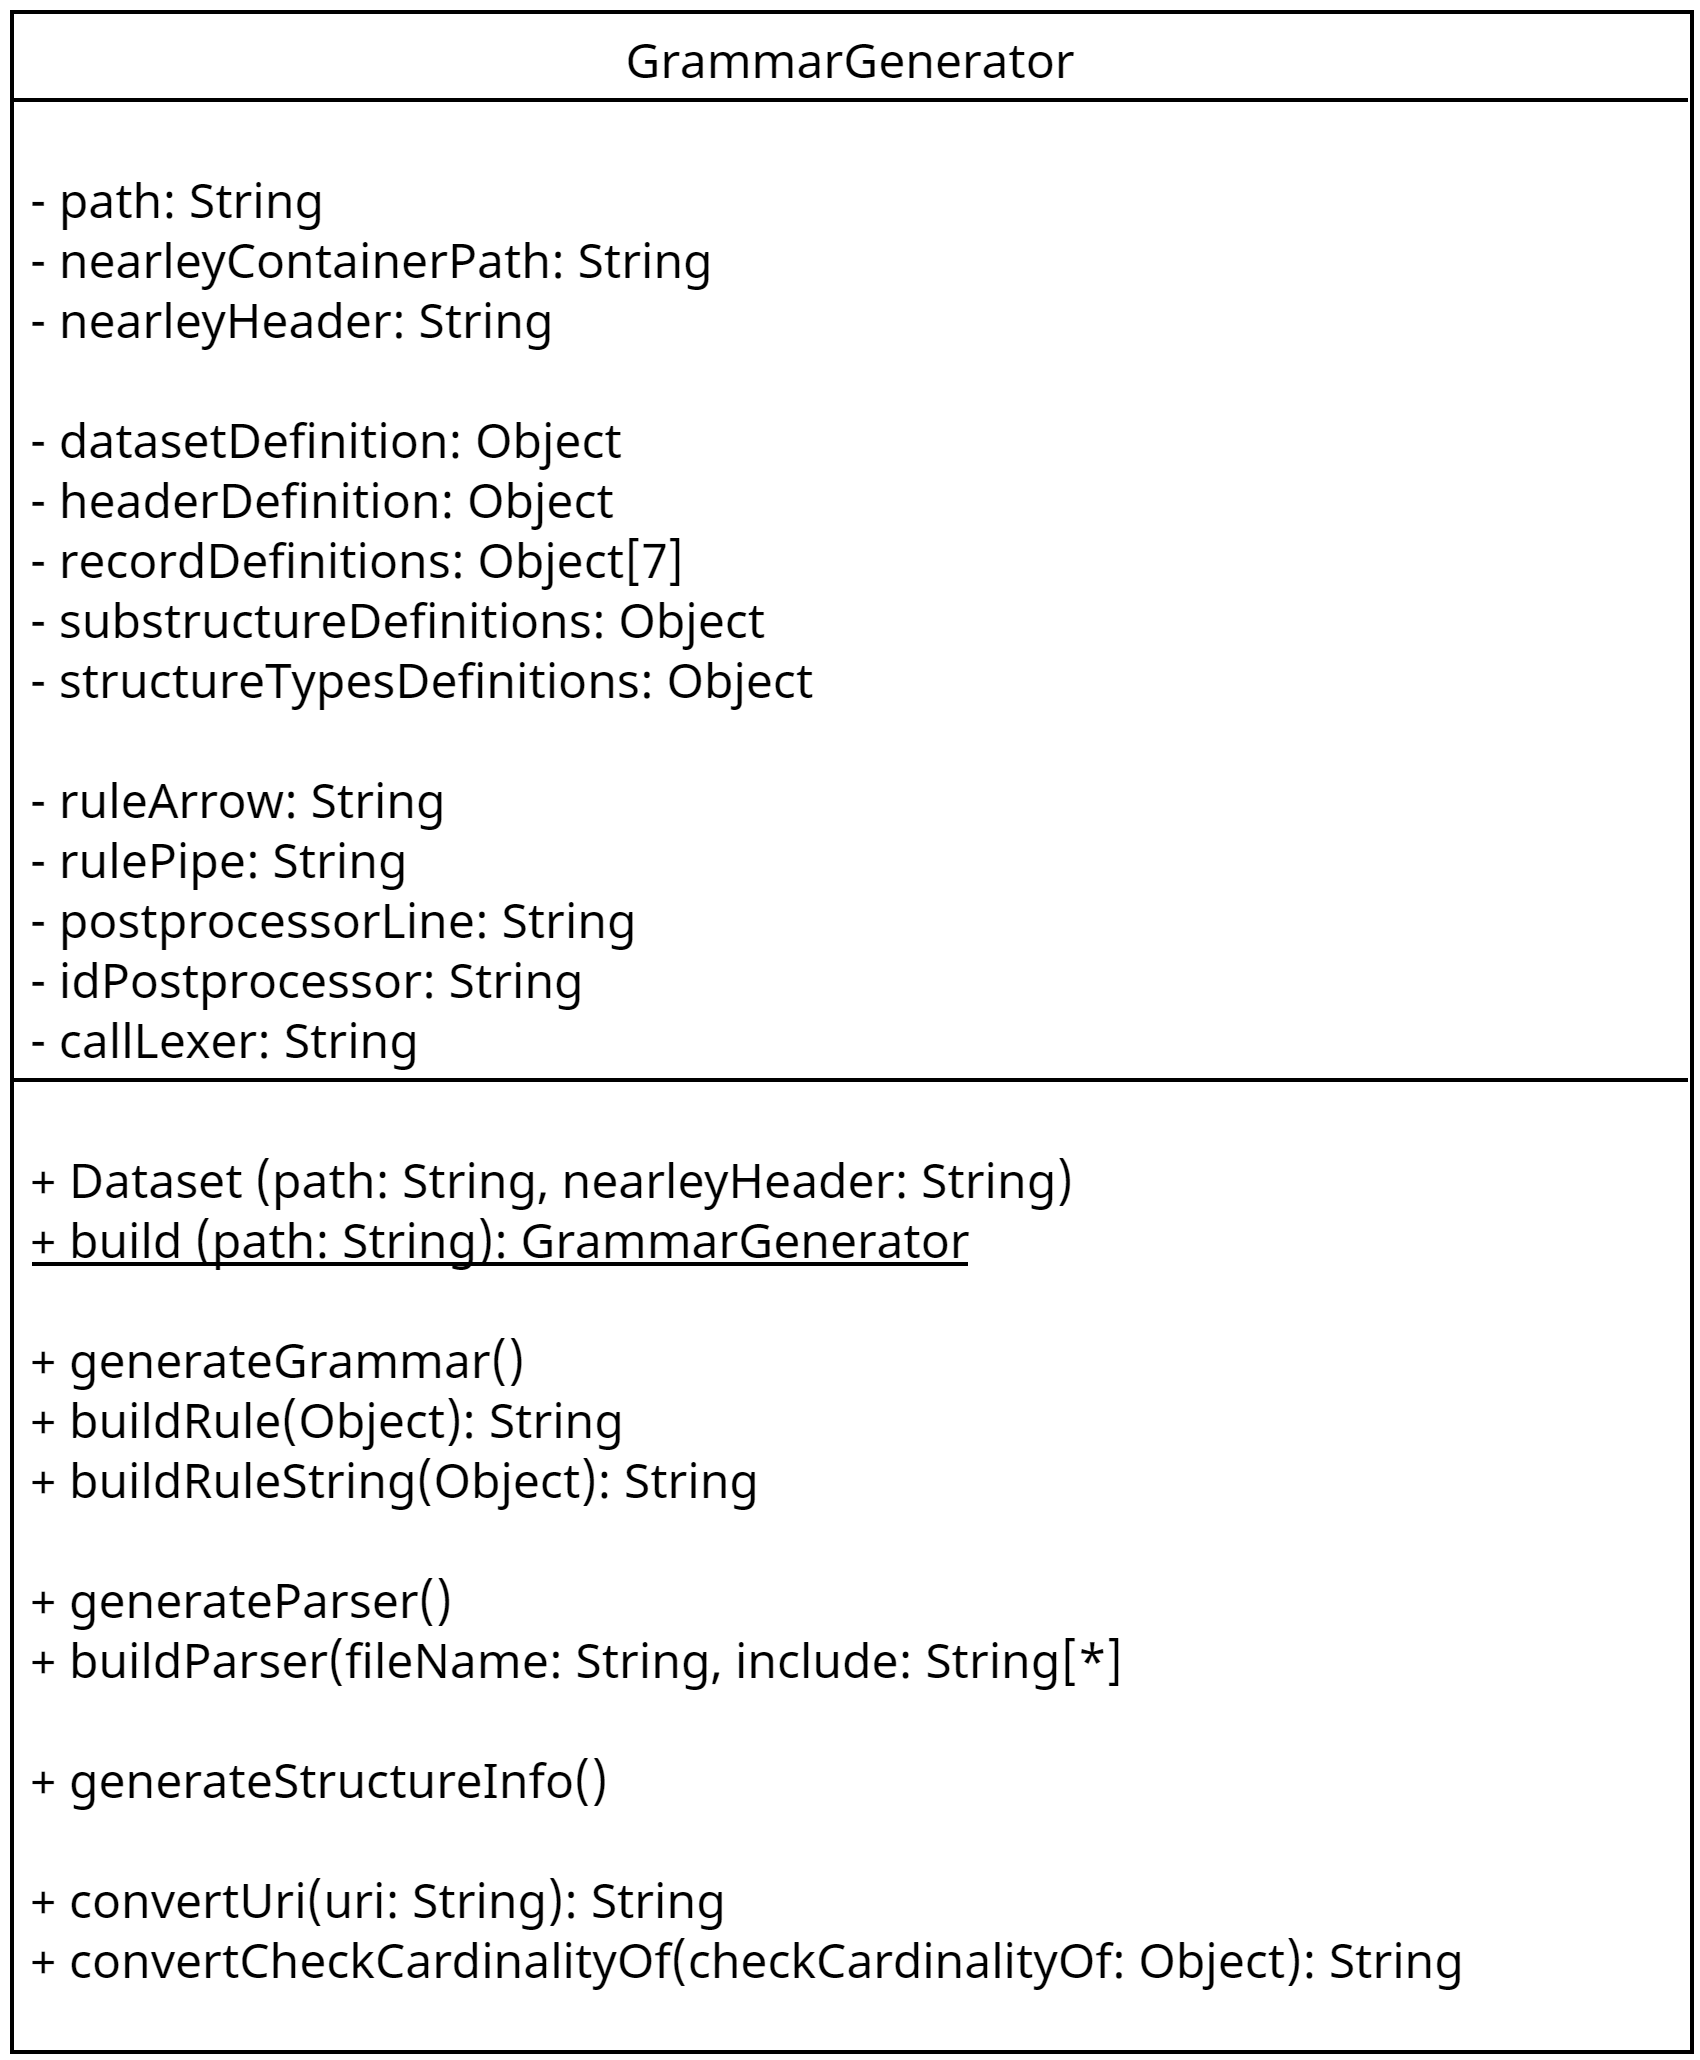
\includegraphics[width=0.7\textwidth]{images/UML_Class_GrammarGenerator.png}
	\caption{UML Klassendiagramm GrammarGenerator}
	\label{fig: UML Klassendiagramm GrammarGenerator}
\end{figure}

\subsection{Definition der Grammatik}
\label{subsec: Implementierung - Grammatik Generator - Definition der Grammatik}
Die Definition der Gedcom Grammatik erfolgt in Form von JavaScript Objekten. Für jede Structure, die in der Gedcom7 Spezifikation definiert ist, wird eine Grammatik Definition erstellt. Folgende Parameter sind in diesen Objekten hinterlegt.

\vspace{1em}
{
	\noindent
	\bgroup
	\def\arraystretch{1.5}%  1 is the default, change whatever you need
	\setlength{\tabcolsep}{18pt}
	\begin{tabular}{|p{2cm}|p{10cm}|}
		\hline
		\textbf{URI} & Die in der Gedcom7 Spezifikation für diese Structure hinterlegte URI. \\
		\hline
		\textbf{lineType} & Der Typ der Line einer Structure (hier wird beispielsweise hinterlegt, ob die Structure einen Cross-Reference-Identifier enthält oder auf andere Structuren verweisen darf). \\
		\hline
		\textbf{Info} & In der Info wird ein Informationstext zu jeder Strucutre hinterlegt. Dieser kann verwendet werden um bei Verwendung der Bibliothek dem Benutzer Informationen über die Bedeutung der Structures zukommen zu lassen.\\
		\hline
		\textbf{Level} & Die Levels unter denen die Structure in einer Gedcom7 Datei auftauchen kann.\\
		\hline
		\textbf{Tag} & Der in der Gedcom7 Spezifikation definierte Tag der Structure.\\
		\hline
		\textbf{Substructs} & Alle Structures, die als Substructure für eine Structure auftauchen können, inkl. der Kardinalität dieser.\\
		\hline
	\end{tabular}
	\egroup
}
\vspace{1em}

Das Definitionsobjekt für einen Family Record ist in Listing \ref{lst: Grammatik Definition Family} dargestellt. Anders als bei den Beispielen aus Abschnitt \ref{sec: Implementierung - Gedcom Grammatik} bei denen nur ein Teil der Substructures betrachtet wurde, handelt es sich hierbei um eine vollständige Definition.
\vspace{1em}
\begin{javascript}{Grammatik Definition eines Family Records}{lst: Grammatik Definition Family}
	{
		uri: 'g7:record-FAM',
		lineType: lineTypes.FAM_RECORD,
		info: 'Structure Info coming soon!',
		level: [0],
		tag: 'FAM',
		substructs: {
			'g7:RESN': '0:1',
			FAMILY_ATTRIBUTE_STRUCTURE: '0:M',
			FAMILY_EVENT_STRUCTURE: '0:M',
			NON_EVENT_STRUCTURE: '0:M',
			'g7:FAM-HUSB': '0:1',
			'g7:FAM-WIFE': '0:1',
			'g7:CHIL': '0:M',
			ASSOCIATION_STRUCTURE: '0:M',
			'g7:SUBM': '0:M',
			LDS_SPOUSE_SEALING: '0:M',
			IDENTIFIER_STRUCTURE: '0:M',
			NOTE_STRUCTURE: '0:M',
			SOURCE_CITATION: '0:M',
			MULTIMEDIA_LINK: '0:M',
			CHANGE_DATE: '0:1',
			CREATION_DATE: '0:1'
		}
	}
\end{javascript}


\subsection{Grammatikgenerierung mit generateGrammar()}
\label{subsec: Implementierung - Grammatik Generator - generateGrammar}
Nach dem in Abschnitt \ref{subsec: Implementierung - Grammatik Generator - Definition der Grammatik} beschriebenen Vorgehen werden Grammatik Definitionen für alle Structuretypes, Substructures und Records, sowie für das gesamte Dataset erstellt. Mit der Funktion \textit{generateGrammar()} werden diese eingelesen, in eine nearley-konforme Zeichenkette konvertiert und anschließend in Form einer Nearley Datei (\textit{.ne}) gespeichert. Die Regeln werden mit der Funktion \textit{buildRuleString()} erzeugt und mit den in der Klasse \textsc{GrammarGenerator} definierten Building-Konstanten zusammengefügt. Ein Beispiel für eine solche Konstante ist der \textit{ruleArrow} der zur Definition einer Regel verwendet wird und als Zeichenkette 
\begin{center}
	''\escape{n}\escape{t} \textendash\textgreater``
\end{center}
kodiert ist. Die so erzeugten Nearley Dateien sind einfach lesbar und liegen in der in Abschnitt \ref{subsec: Implementierung - Gedcom Grammatik - Gedcom7 Syntax in Nearley} Form vor. Alle so erstellten Nearley Dateien werden im mit \textit{path} spezifizierten Pfad im Verzeichnis ''\textit{path/nearley/}`` abgelegt.

\subsection{Parsergenerierung mit generateParser()}
\label{subsec: Implementierung - Grammatik Generator - generateParser}
Mit der Funktion \textit{generateParser()} werden die Nearley Grammatiken für alle Records und das gesamte Dataset zu Nearley Parsern kompiliert. Dazu stellt Nearley die Funktion 
\begin{center}
	nearleyc  \textit{inputPath} -o \textit{outputPath}
\end{center}
bereit, mit eine Nearley Datei eingelesen und im spezifizierten Pfad kompiliert werden kann. Das Erstellen von Parsern für die Records ist notwendig, da die Nearley Parser für die Syntaxüberprüfung nach Änderung eines Records verwendet werden. Würde nur ein allgemeiner Dataset-Parser erstellt werden, müsste nach jeder Änderung das komplette Dataset überprüft werden, obwohl nur ein Record verändert wurde. 

Im ersten Schritt der Funktion \textit{generateParser()} werden die Include-Statements vorbereitet, die z.B. die Definition der Datentypen enthalten. Anschließend wird für die Record- und Dataset-Grammatiken die Funktion \textit{buildParser()} aufgerufen, die in Listing \ref{lst: GrammarGenerator Funktion buildParser()} dargestellt ist. Hier werden die mit \textit{generateGrammar()} erzeugte Grammatik, die Include-Statements und der Nearley Header in einer Container Datei \textit{NearleyContainer.ne} zusammengefügt. Diese Container Datei wird anschließend zu dem entsprechenden Parser kompiliert und im mit \textit{path} spezifizierten Pfad im Verzeichnis ''\textit{path/parser/}`` abgelegt.
\vspace{0.9em}
\begin{javascript}{Funktion buildParser() des Grammatik Generators}{lst: GrammarGenerator Funktion buildParser()}
	// build nearley-file with include statements and NearleyHeader
	async buildParser (fileName, include) {
		// string representation of the grammar to be compiled
		let fileStr = '';
		// add given include statements
		for (const file of include) {
			fileStr += `@include "../grammar/nearley/${file}"\n`;
		}
		// add nearley header
		fileStr += this.nearleyHeader;
		
		// overwrite content of NearleyContainer file
		await fs.writeFile(this.nearleyContainerPath, fileStr);
		// read grammar of given file
		const grammar = await fs.readFile(`${this.path}nearley/${fileName}.ne`, { encoding: 'utf8' });
		// append grammar to NearleyContainer file
		fs.appendFile(this.nearleyContainerPath, grammar);
		
		// compile composed NearleyContainer.ne file to nearley parser
		await exec(`npx nearleyc ${this.nearleyContainerPath} -o ${this.path}parser/${fileName}Parser.js`);
	}
\end{javascript}
%========================================================================================
% SECTION: GEDCOM STRUKTUR
%========================================================================================
\section{Gedcom Struktur}
\label{sec: Implementierung - Gedcom Struktur}
Die Struktur einer Gedcom7 Datei wird in der Bibliothek \textit{gedcom7.js} mit Hilfe der Klasse \textsc{Dataset} abgebildet, die alle Gedcom Structures verwaltet, die in Form der gleichnamigen Klasse \textsc{Structure} vorliegen. Structures werden in \textit{gedcom7.js} entweder als allgemeine Instanz der Klasse \textsc{Structure} (z.B. eine HUSB-Structure), als \textsc{Record} (z.B. ein Family Record) oder als \textsc{Datatype Structure} (z.B. eine DATE-Structure) repräsentiert. 

\subsection{Klasse \textsc{Structure}}
\label{subsec: Implementierung - Gedcom Struktur - Klasse Structure}
Die Klasse \textsc{Structure} ist die Überklasse aller Klassen zur Structure-Verwaltung, d.h. Records und Datatyp Structures erben alle Methoden und Eigenschaften von \textsc{Structure}. Diese Methoden und Eigenschaften sind in Abbildung \ref{fig: UML Klassendiagramm Structure} abgebildet. Eine Instanz der Klasse \textsc{Structure} hält alle Informationen über eine Line bereit (URI, Level, Tag, Xref, lineValue, Typ des LineValues, EOL-Zeichen). Außerdem werden Referenzen zu allen Substructures, der Superstructure, dem Record mit dem die Structure assoziiert wird, sowie zum Dataset in dem die Structure enthalten ist bereitgestellt. Außerdem übernimmt die Klasse \textsc{Structure} vier zentrale Aufgaben zur Verwaltung von Gedcom7 Informationen, die von der Klasse \textsc{Dataset} angestoßen werden können.

\begin{figure}[h]
	\centering
	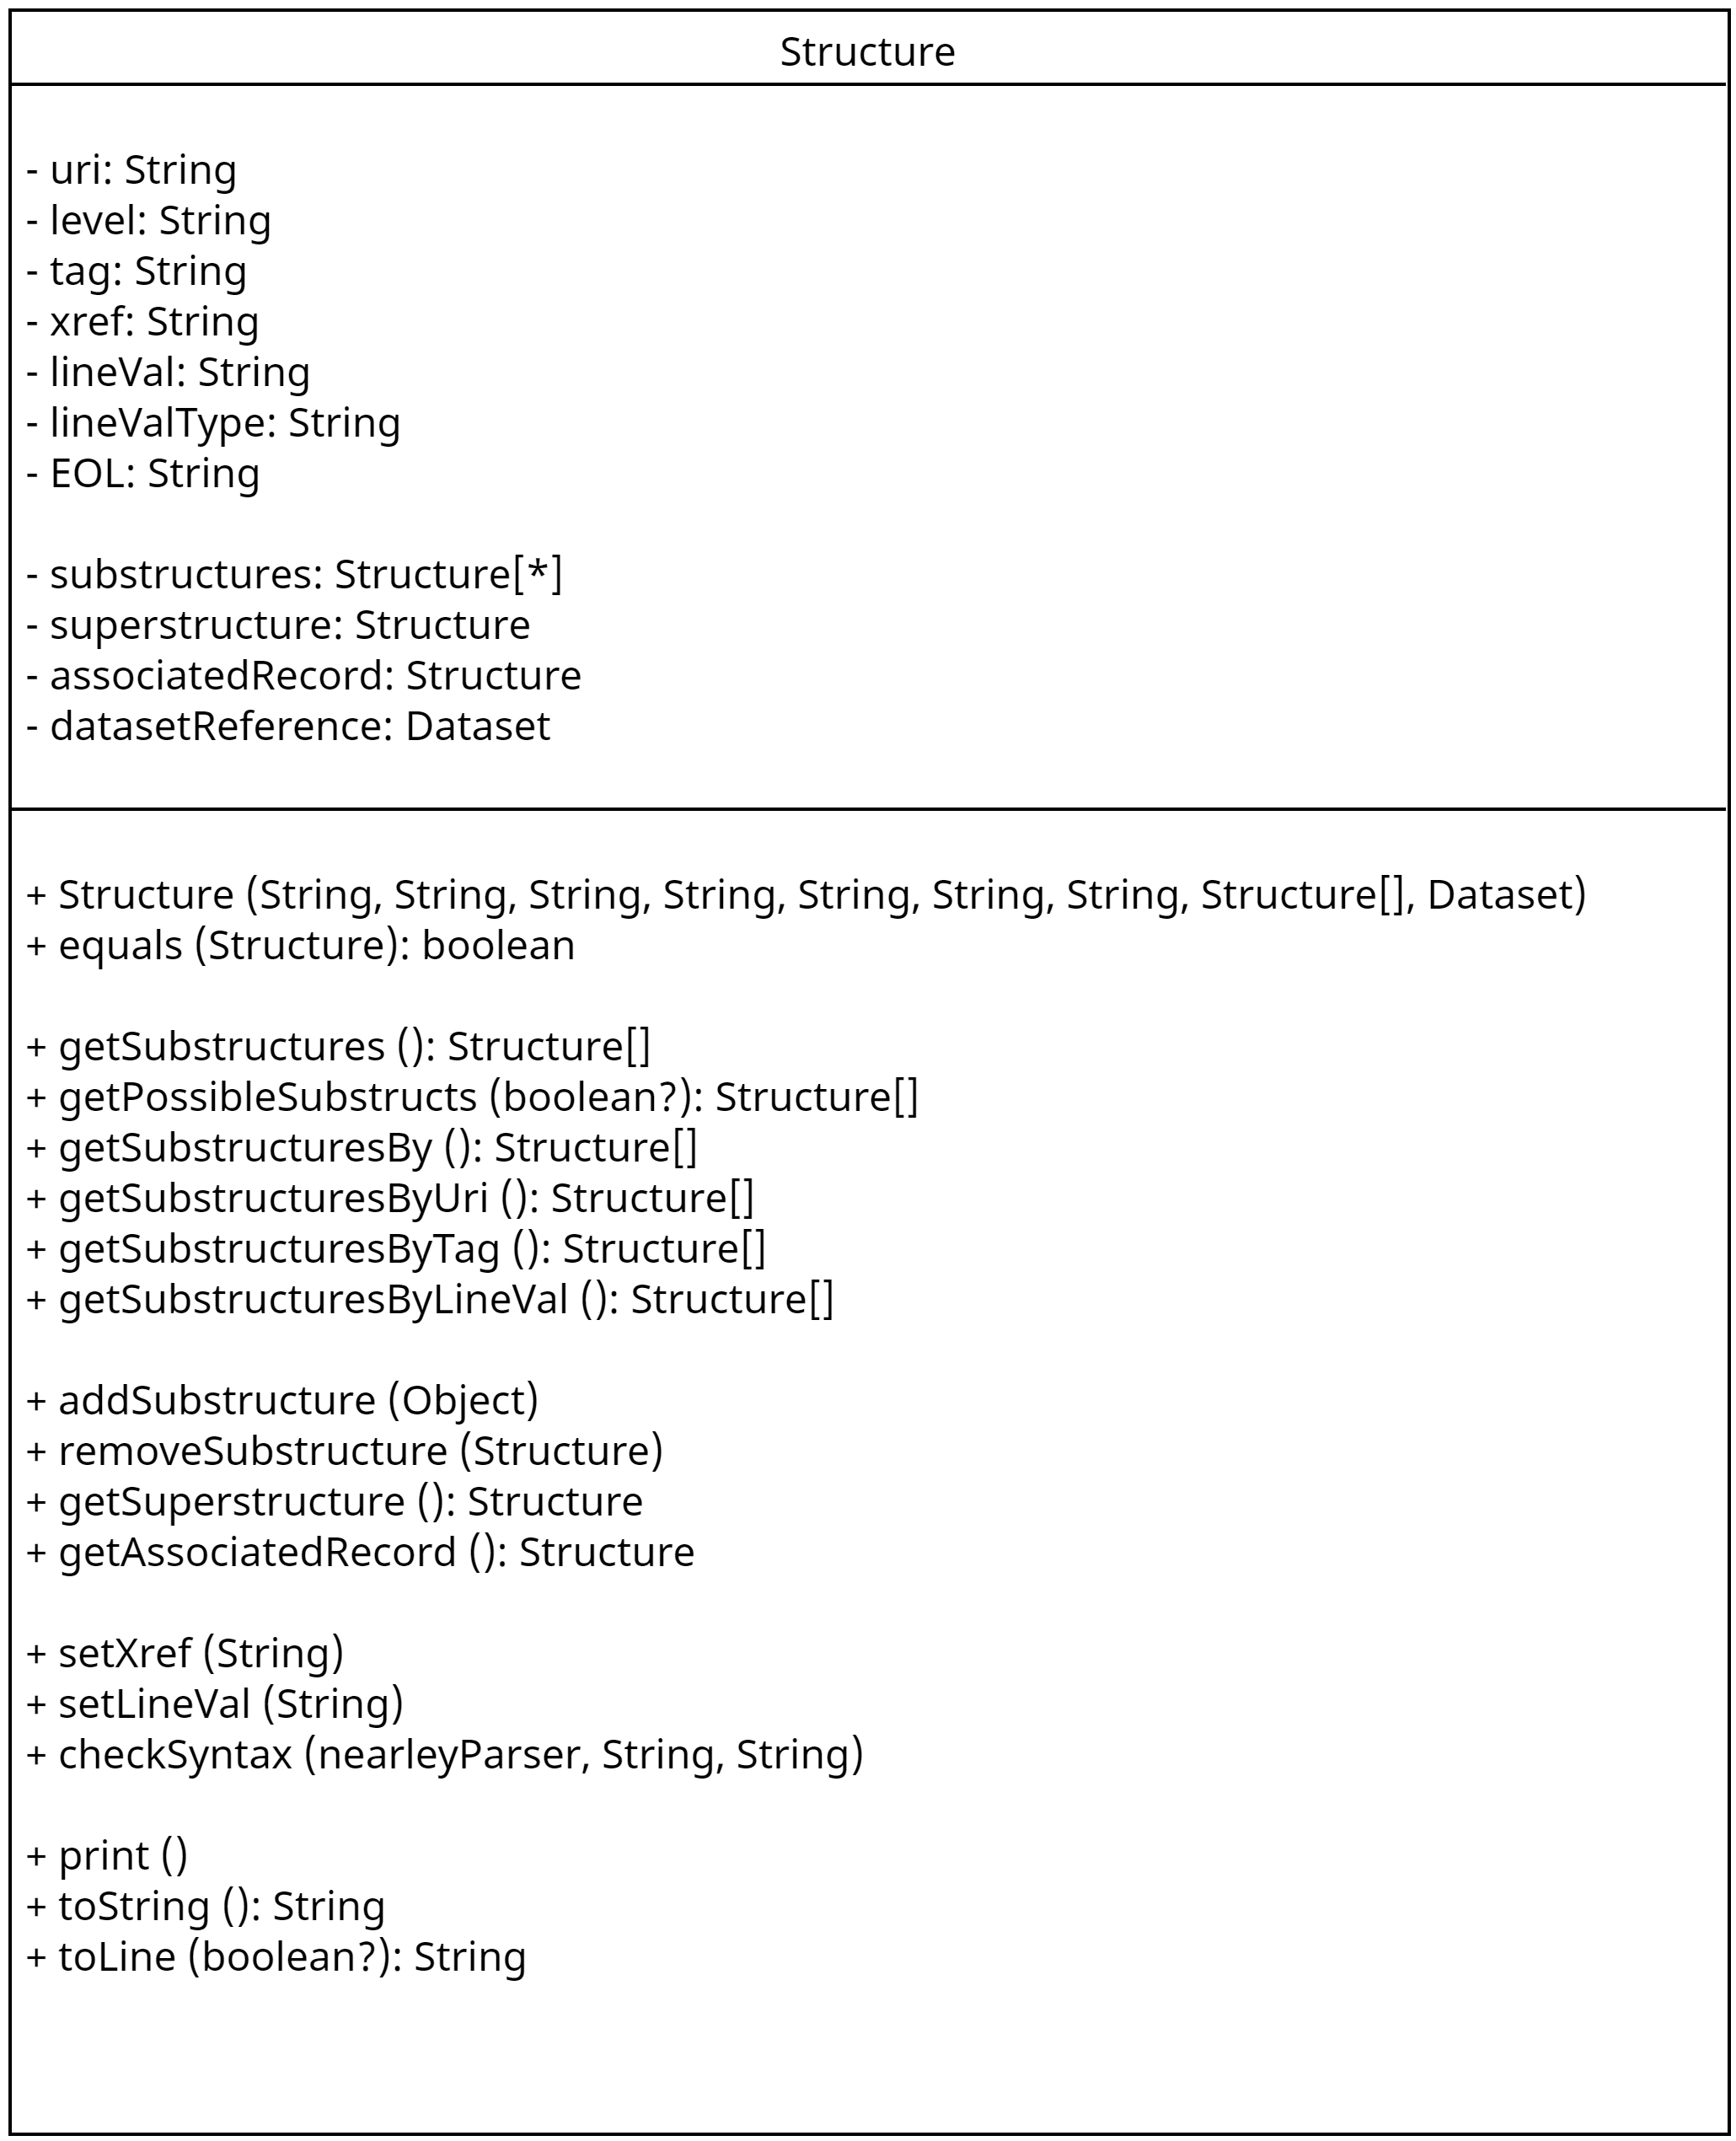
\includegraphics[width=0.75\textwidth]{images/UML_Class_Structure.png}
	\caption{UML Klassendiagramm Structure}
	\label{fig: UML Klassendiagramm Structure}
\end{figure}

\vspace{1em}
\textbf{1. Finden von Substructures} \vspace{0.5em} \\
Eine der wichtigsten Aufgaben der Klasse \textsc{Structure} ist es, eigene Substructures zu suchen und zu finden. Dazu werden die Methoden \textit{getSubstructuresByUri()}, \textit{getSubstructuresByTag()} und \textit{getSubstructuresByLineVal()} bereitgestellt, die alle Substructures zurückgeben, die einem Suchkriterium genügen, das abhängig von der Methode eine Gedcom7 URI, ein Gedcom7 Tag oder einen LineValue darstellen. Über den Parameter \textit{recursive} kann spezifiziert werden, ob nur direkte Substructures (also mit einem um $1$ inkrementierten Level) gesucht oder ebenfalls alle Substructures von Substructures rekursiv durchsucht werden sollen. Sollen einfach alle Substructures einer Structure ohne Suchkriterium zurückgegeben werden, kann die Methode \textit{getSubstructures()} verwendet werden.


In vielen Anwendungsfällen kann es zudem von Interesse sein, welche Structures als Substructure in Frage kommen (also welche Structures in der Gedcom7 Spezifikation als potentitelle Substructures definiert sind). Ein Beispiel hierfür wäre ein Benutzer, der einen Family Record verwaltet und herausfinden möchte, welche weiteren Informationen angegeben werden können. Für diesen Fall wird die Methode \textit{getPossibleSubstructs()} bereitgestellt, die die Gedcom7 URIs aller Structures zurückgibt, die als Substructure auftreten können. Über den boolschen Parameter \textit{checkCardinalityFlag} kann spezifiziert werden, ob die Kardinalität überprüft werden soll, d.h. ob nur diejenigen URIs bereitgestellt werden sollen, die beim Hinzufügen nicht zu einem CardinalityError führen. 
\newpage
\vspace{1em}
\textbf{2. Hinzufügen und Entfernen von Substructures} \vspace{0.5em} \\
Die Klasse \textsc{Structure} stellt die Methode \textit{addSubstructure()} zur Verfügung, um einer Instanz der Klasse eine Substructure hinzuzufügen. Der Ablauf dieser Operation ist in einem Aktivitätsdiagramm in Abbildung \ref{fig: UML Aktivität addSubstructure} dargestellt. Alle benötigten Informationen über die Substructure werden als Parameter \textit{StructureParameter} übergeben. In der Methode werden diese Informationen extrahiert und auf Basis dessen eine neue Instanz der Klasse \textsc{Structure} erstellt. Dieses Objekt wird in das Dataset eingefügt indem alle nötigen Referenzen angepasst werden und das Objekt Teil so der Gedcom Struktur wird. Anschließend wird die Syntax des Records überprüft, in den die neue Structure eingefügt wurde um zu überprüfen, ob immernoch ein Gedcom7 konformes Dataset vorliegt. Ist dies der Fall wird im Dataset überprüft, ob undefinierte Cross-Reference-Identifier vorliegen. 


Falls eine dieser Überprüfungen fehlschlägt, wird die Substructure über die Methode \textit{removeSubstructure()} aus dem Dataset entfernt, indem die gleichnamige Methode der Klasse \textsc{Dataset} aufgerufen wird (siehe Abschnitt \ref{subsec: Implementierung - Gedcom Struktur - Klasse Dataset}).
\begin{figure}[h]
	\centering
	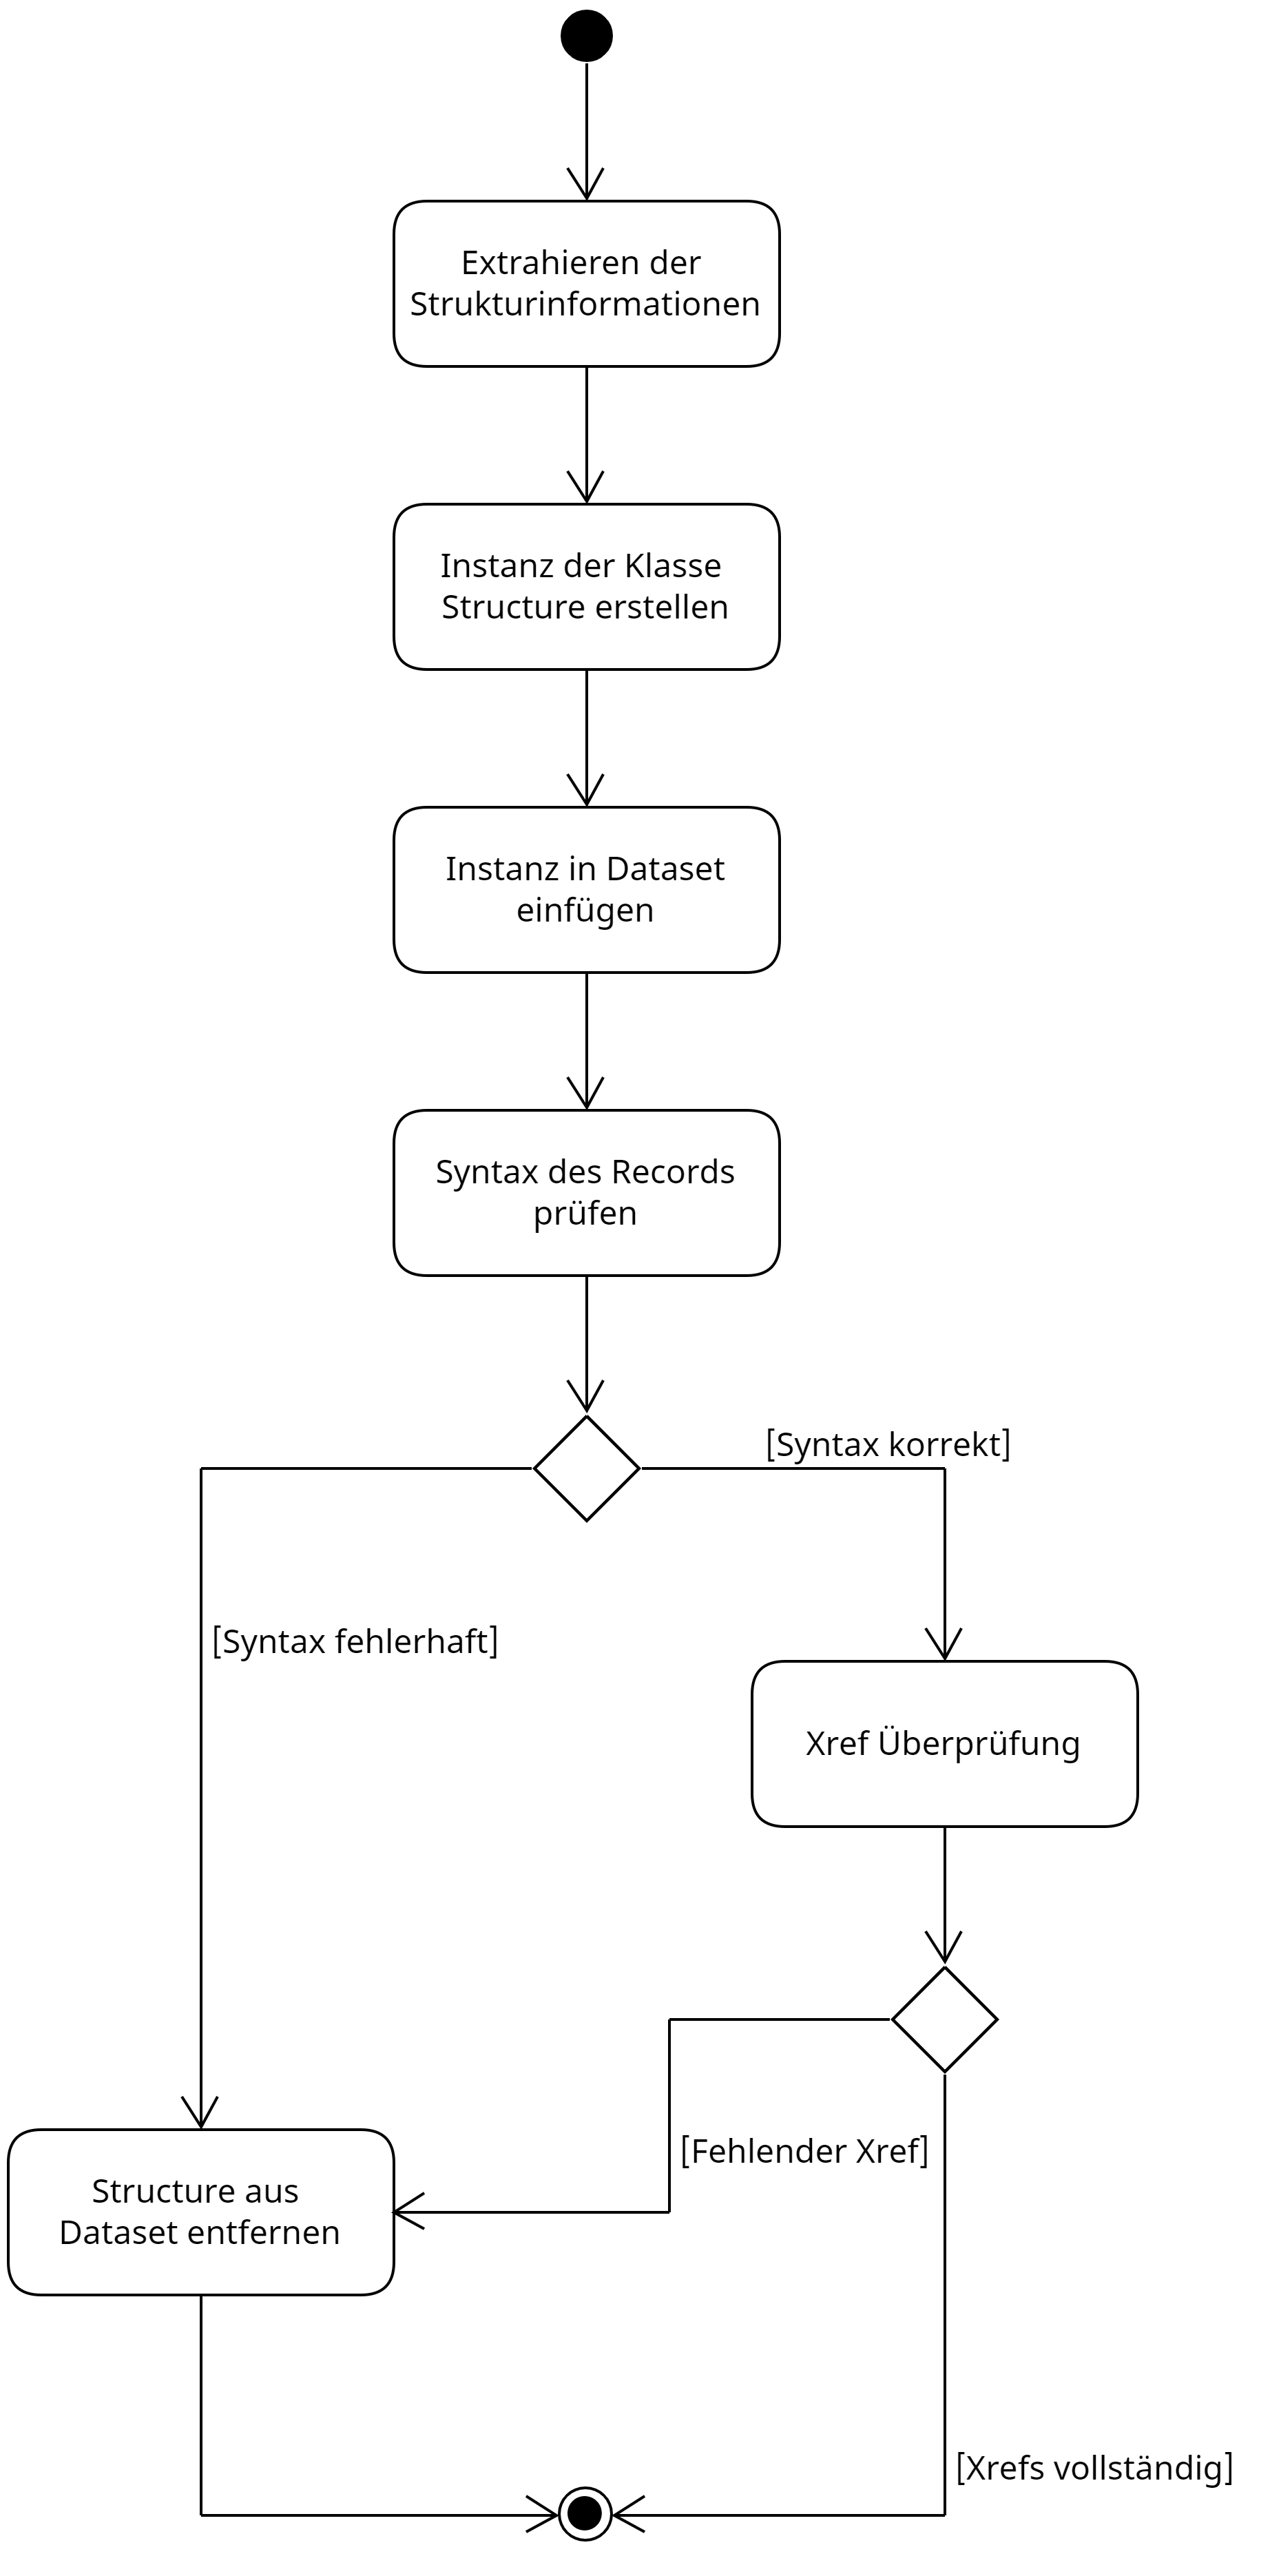
\includegraphics[width=0.45\textwidth]{images/UML_Activity_AddSubstruct.png}
	\caption{UML Aktivitätsdiagramm der Methode \textit{addSubstructure()}}
	\label{fig: UML Aktivität addSubstructure}
\end{figure}

\textbf{3. Ändern des LineValues} \vspace{0.5em} \\
Der LineValue einer Instanz der Klasse \textsc{Structure} kann über die Methode \textit{setLineVal()} verändert werden (siehe Abbildung \ref{fig: UML Aktivität setLineVal}). Die Eigenschaft \textit{lineVal} des \textsc{Structure} Objekts wird auf den als Parameter übergebenen Wert gesetzt und anschließend wird die Syntax des entsprechenden Records überprüft, um zu kontrollieren, dass der neue LineValue syntaktisch korrekt ist.
Handelt es sich um eine Structure, die einen LineValue des Typs \textit{Xref}\footnote{Ein Beispiel hierfür wäre die HUSB-Structure, die auf einen Individual Record verweist.} besitzt, also auf eine andere Structure verweist, muss ebenfalls \textit{Xref-Map} des Datasets aktualisiert werden. In dieser Map werden alle Verweise über Cross-Reference-Identifier, die im Dataset vorkommen, verwaltet. Werden nach der Veränderung des LineValues ein Syntaxfehler oder undefinierte Cross-Reference-Identifier gefunden, muss der LineValue auf den Ursprungswert zurückgesetzt werden. 

Da auch ein leerer LineValue syntaktisch korrekt sein kann, wird im letzten Schritt das Dataset nach leeren Structures durchsucht, die dann entfernt werden. Ein Beispiel hierfür wäre die MARR-Structure aus dem Family Record in Listing \ref{lst: family record example}. Würde hier der DATE-Structure ein leerer Wert zugewiesen werden, würde dies in der Structure
\begin{lstlisting}[frame=none]
					   1 MARR
					   2 DATE
\end{lstlisting}
resultieren. Diese Structure enthält keinerlei Informationen und kann daher entfernt werden.
 
\begin{figure}[h]
	\centering
	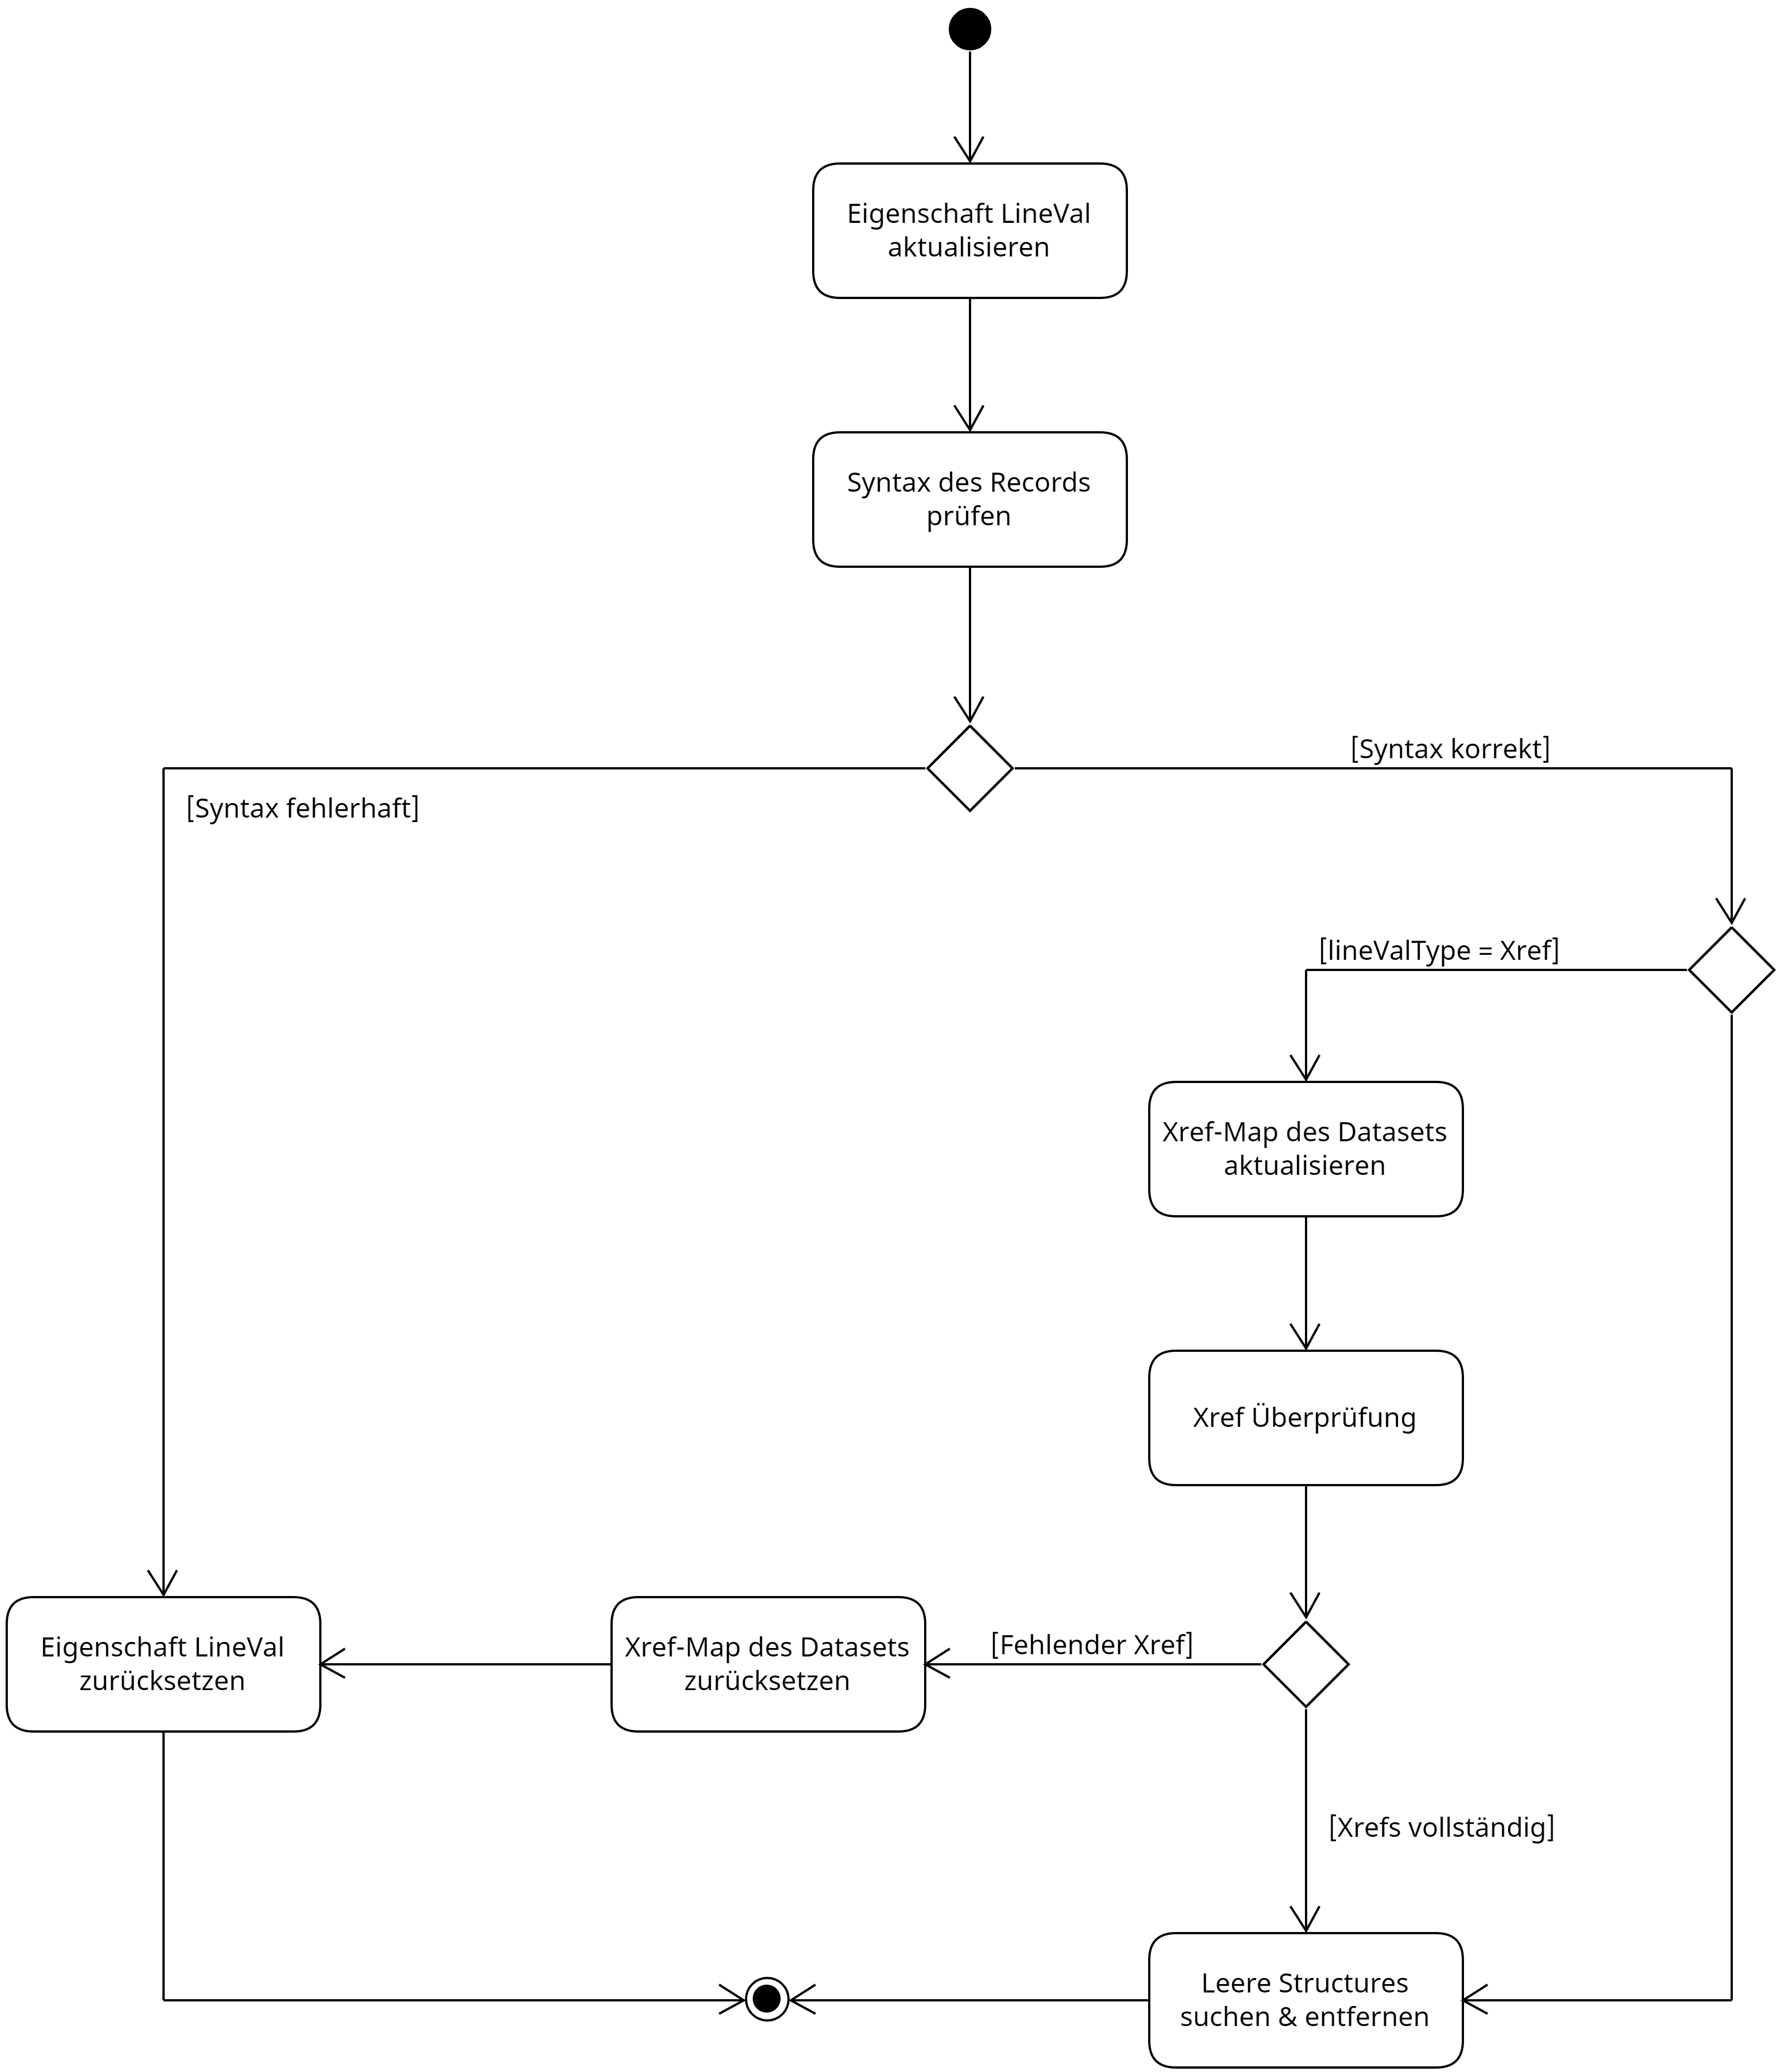
\includegraphics[width=0.76\textwidth]{images/UML_Activity_SetLineVal.png}
	\caption{UML Aktivitätsdiagramm der Methode \textit{setLineVal()}}
	\label{fig: UML Aktivität setLineVal}
\end{figure}


\subsection{Klasse \textsc{Record}}
\label{subsec: Implementierung - Gedcom Struktur - Klasse Record}
Die Klasse \textsc{Record} ist die Vaterklasse für Family, Individual, Header, Multimedia, Repository, SharedNote, Source und Submitter und definiert eine Methode zur Syntaxüberprüfung eines Records. Dazu wird der entsprechende Nearley-Parser, der mit dem in Abschnitt \ref{sec: Implementierung - Grammatik Generator} beschriebenen \textsc{GrammarGenerator} erstellt wurde, eingebunden. Dieser bekommt alle Lines des Records kodiert als Zeichenkette als Eingabe und überprüft ob alle Structures syntaktisch korrekt sind.


Des Weiteren stellt die Klasse \textsc{Record} Methoden zur Verfügung, um Informationen aus Structures, die von mehreren Records geteilt werden, zu extrahieren und in gebündelter Form auszugeben. Ein Beispiel hierfür sind die Identifier-Structures, die genutzt werden um Structures oder ihre Inhalte eindeutig zu identifizieren. Die Klasse \textsc{Record} stellt dafür die Mehtode \textit{extractIdentifierStructures()} zur Verfügung, mit der alle Identifier-Structures eines Records gesucht und in gebündelt zurückgegeben werden. Wie in Listing \ref{lst: extractIdentifier Funktion} dargestellt, wird die Methode \textit{getSubstructuresByUri()} (siehe Abschnitt \ref{subsec: Implementierung - Gedcom Struktur - Klasse Structure}) verwendet, um alle Identifier-Structures des Records zu finden. Anschließend werden alle Informationen extrahiert und im JSON-Format zurückgegeben. 
\vspace{1em}
\begin{javascript}{Methode \textit{extractIdentifierStructures()} der Klasse \textsc{Record}}{lst: extractIdentifier Funktion}
	// extracts content of IDENTIFIER_STRUCTURE
	//  -> Each value provides an identifier for a structure or its subject, and each is different in purpose
	extractIdentifierStructures () {
		// REFN (Reference) is user-defined number or text that the submitter uses to identify the superstructure
		const references = this.getSubstructuresByUri('g7:REFN', false);
		// UID is a globally-unique identifier of the superstructure, to be preserved across edits
		const UIDs = this.getSubstructuresByUri('g7:UID', false);
		// EXID is an identifier maintained by an external authority that applies to the subject of the structure.
		const externalIdentifier = this.getSubstructuresByUri('g7:EXID', false);
		
		if (references || UIDs || externalIdentifier) {
			return {
				references: references?.map((ref) => {
					return {
						reference: ref.lineVal || null,
						type: ref.getSubstructuresByUri('g7:TYPE', false)[0]?.lineVal || null
					};
				}) || null,
				uniqueIdentifier: UIDs?.map((uid) => uid.lineVal),
				externalIdentifier: externalIdentifier?.map((exid) => {
					return {
						id: exid.lineVal || null,
						type: exid.getSubstructuresByUri('g7:EXID-TYPE', false)[0]?.lineVal || null
					};
				}) || null
			};
		}
		return null;
	}	
\end{javascript}
\vspace{1em}
Alle Eigenschaften und Methoden der Klasse \textsc{Record} sind in Abbildung \ref{fig: UML Klassendiagramm Record} dargestellt.
\begin{figure}[h]
	\centering
	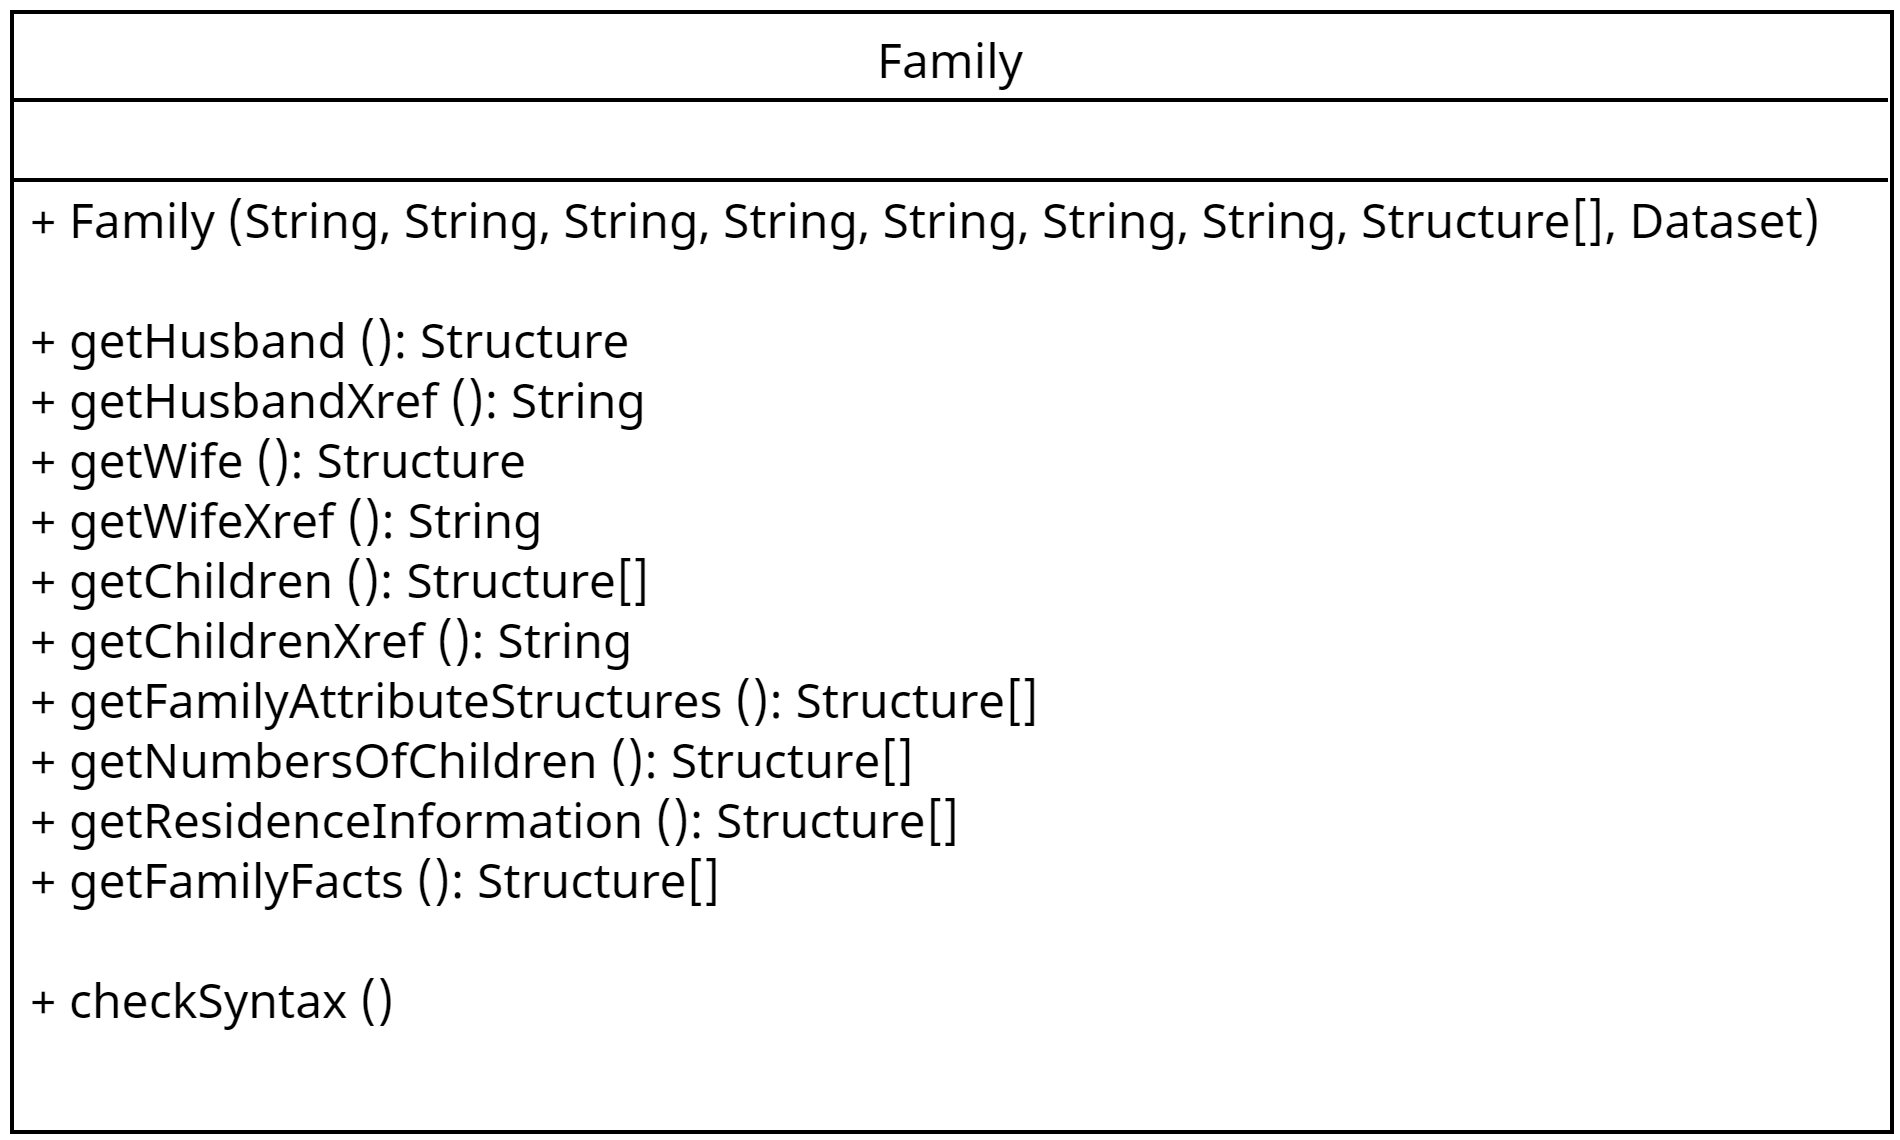
\includegraphics[width=0.8\textwidth]{images/UML_Class_Record.png}
	\caption{UML Klassendiagramm Record}
	\label{fig: UML Klassendiagramm Record}
\end{figure}

\label{subsec: Implementierung - Gedcom Struktur - Klasse Family}
\subsection{Klasse \textsc{Family}}
Ein Ziel bei der Erstellung der Bibliothek \textit{gedcom7.js} war es, eine Grundlage für die Verarbeitung von Gedcom7 Dateien zu kreieren, die in zukünftigen Arbeiten erweitert werden kann. Daher wurde für diese Arbeit nur die Klasse \textsc{Family} für den Family Record vollständig implementiert. Die Klassen für alle weiteren Records können analog zu dem hier beschrieben Vorgehen erstellt werden, um die Gedcom7 Spezifikation komplett abzubilden. 


Die Klasse \textsc{Family} ruft die Methode \textit{checkSyntax()} der Vaterklasse \textsc{Record} mit der Family Grammatik auf. Des Weiteren werden Methoden zur einfachen Verarbeitung von Informationen aus einem Family Record bereitgestellt. Ist ein Anwender beispielsweise an Informationen über die Kinder einer Familie interessiert, müsste er die Gedcom7 Spezifikation studieren, alle Structures die Informationen über ein Kind bereithalten können nacheinander suchen und dann alle Informationen zusammenfügen. Um diese Arbeit zu erleichtern, werden in der Bibliothek \textit{gedcom7.js} die in Abbildung \ref{fig: UML Klassendiagramm Family} aufgeführten Convenience-Methoden bereitgestellt. Ein Beispiel hierfür ist die in Listing \ref{lst: extractIdentifier Funktion} abgebildete Methode \textit{getChildrenInformation()}, mit der alle Informationen über die Kinder einer Familie extrahiert werden können. Dazu werden die entsprechenden Strukturen über die Methode \textit{getSubstructuresByUri} gesucht und im JSON-Format zurückgegeben. Alle Methoden und Eigenschaften der Klasse \textsc{Family} sind in Abbildung \ref{fig: UML Klassendiagramm Family} aufgeführt.
\vspace{1em}
\begin{javascript}{Methode \textit{extractIdentifierStructures} der Klasse \textsc{Record}}{lst: extractIdentifier Funktion}
	// returns information about the children of this family
	getChildrenInformation () {
		const famNCHI = this.getSubstructuresByUri('g7:FAM-NCHI', false)[0];
		const famEventDetail = this.extractFamilyEventDetail(famNCHI);
		
		if (famNCHI) {
			return {
				numberOfChildren: Number.parseInt(famNCHI.lineVal) || null,
				type: famNCHI.getSubstructuresByUri('g7:TYPE', false)[0]?.lineVal || null,
				parentInformation: famEventDetail?.parentInformation || null,
				eventDetails: famEventDetail?.eventDetails || null
			};
		}
		return null;
	}
\end{javascript}

\begin{figure}[h]
	\centering
	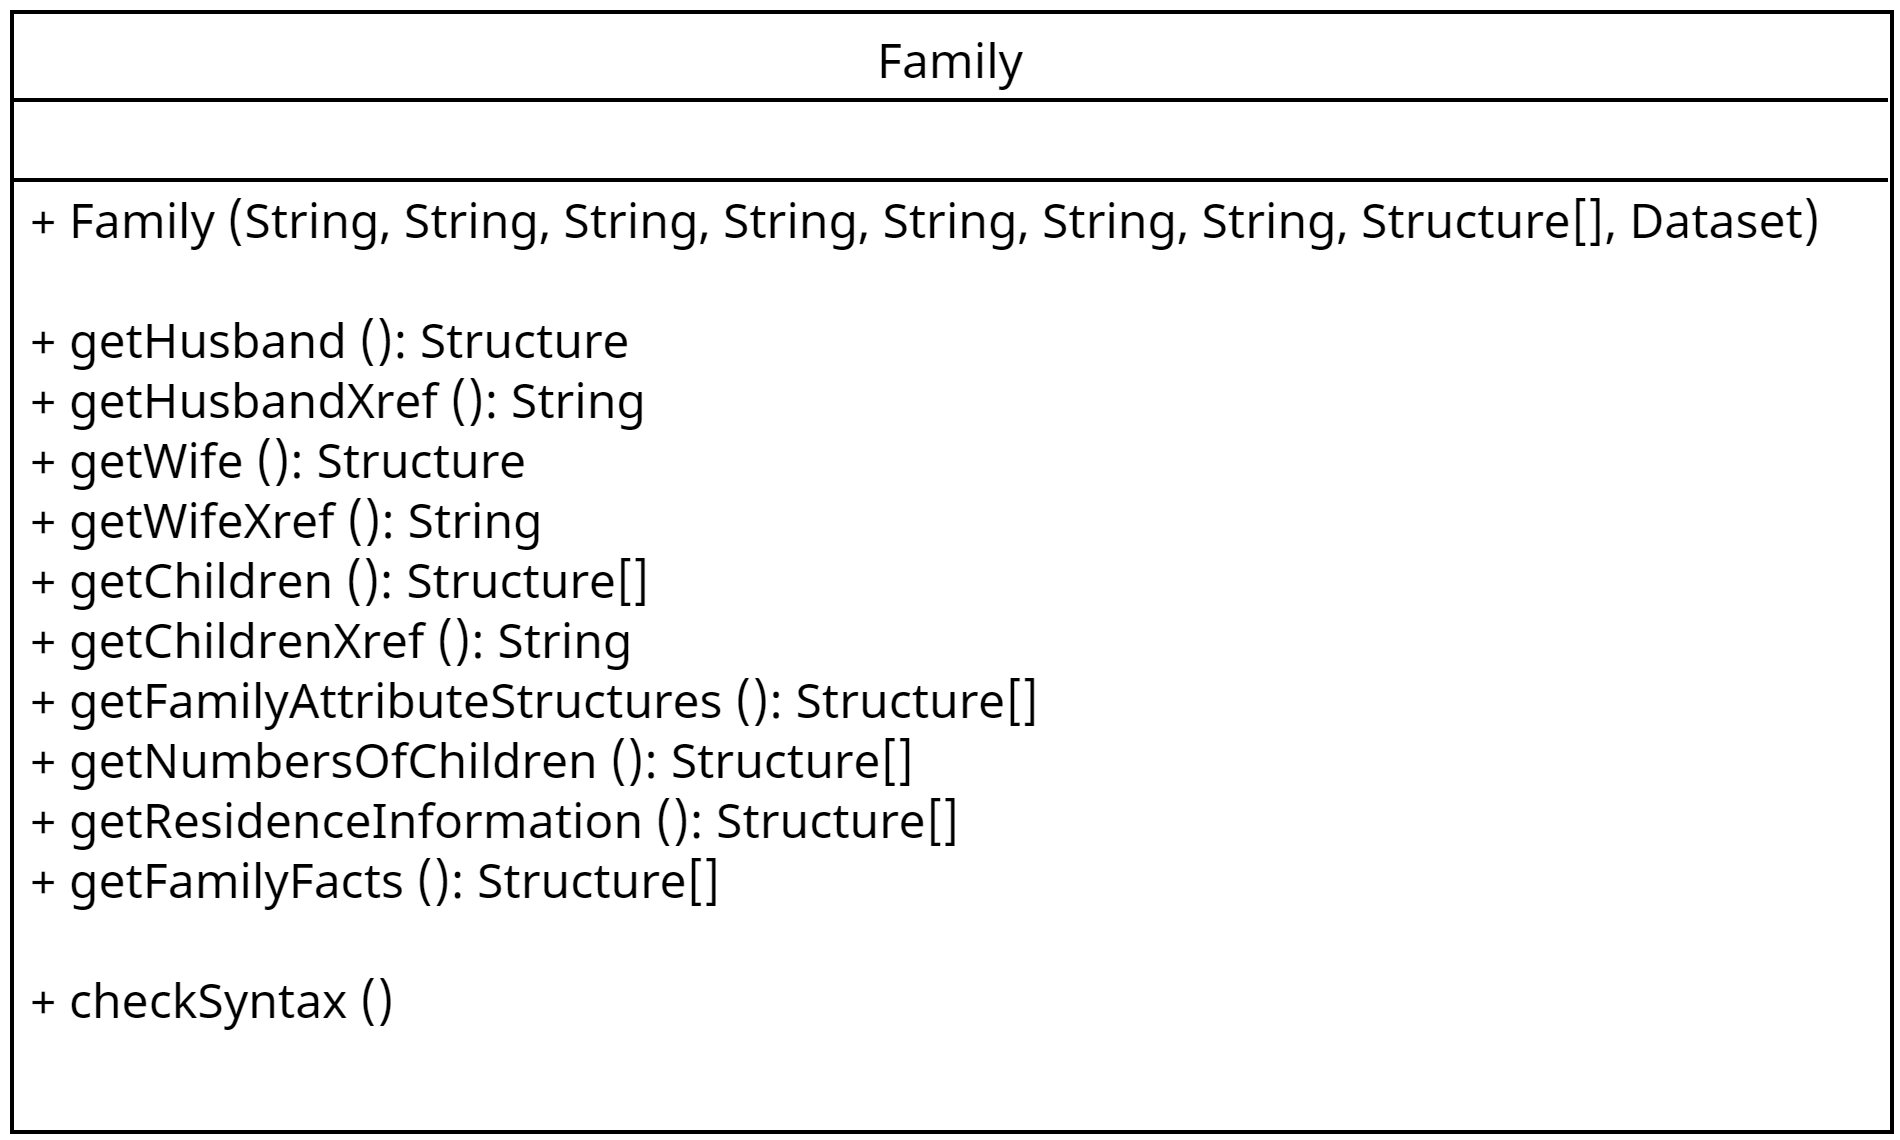
\includegraphics[width=0.8\textwidth]{images/UML_Class_Family.png}
	\caption{UML Klassendiagramm Family}
	\label{fig: UML Klassendiagramm Family}
\end{figure}
\newpage
\subsection{Datatype Structures: \textsc{GedcomDate} Klasse}
Um besser mit den Datentypen der GEDCOM-Spezifikation innerhalb der Bibliothek umgehen zu können, 
wurden Datentyp-Strukturen eingeführt und die Klasse \textsc{GedcomDate} exemplarisch implementiert.

Diese soll als Vorlage für weitere GEDCOM-Datentypen, oder erweiterte Datentypen, genutzt werden.
Nach dem erfolgreichen Parsen, werden die Klassen für die \textit{Records} und \textit{Structures}, 
sowie auch die Datentyp-Strukturen erstellt.

Wenn vom Nearley-Parser die GEDCOM-Typen \textit{DateValue}, \textit{DatePeriod} oder \textit{DateExact}
erkannt werden, wird die Klasse \textsc{GedcomDate} mit den entsprechenden Line-Parametern instanziiert.
Beim Initialisieren der \textsc{GedcomDate}-Klasse wird das spezifikationskonforme Datum, mit Hilfe der 
Datums-Bilbliothek \textit{date-fns}, in ein JavaScript-Date-Objekt umgewandelt.
Je nach GEDCOM-Date-Typ wird das Datum nur in das Attribut \textit{startDate} oder auch und in das Attribut
\textit{endDate} der Klasse GedcomDate, gespeichert. \\
Die Klasse \textsc{GedcomDate} bietet eine Methode \textit{getDateObject()}, in der das GEDCOM Datum 
als JavaScript-Date-Objekt mit Metadaten zum Date-Typ zurückgegeben wird.
Diese Methode ist in Listing \ref{lst: getDateObject function} abgebildet. Es wird zunächst kontrolliert,
ob eine Datumsspanne oder ein einzelnes Datum vorliegt. Anschließend wird das result-Objekt konditional
mit den vorhandenen Properties gefüllt und zurückgegeben. Das start/endDate beeinhaltet ebenfalls die Uhrzeit, 
welche in GEDCOM als Substructure der Date-Structure angegeben werden kann.

\newpage

\begin{javascript}{Funktion getDateObject() der Klasse \textsc{GedcomDate}}{lst: getDateObject function}
	// public method to get the date as an object 
	// with a descriptor (in case of a special date)
    getDateObject() {
        // determine if the date is a single date or a date range
        const isDateRange = this.startDate !== null && this.endDate !== null;
        
        // create result object with conditionally added properties
        const result = {
            type: this.lineValType,
            ...(isDateRange && { startDate: this.startDate, endDate: this.endDate }),
            ...(!isDateRange && { date: this.startDate }),
            ...(this.descriptor && { descriptor: this.descriptor }),
            ...(this.description && { description: this.description }),
            ...(this.calendar && { calendar: this.calendar }),
            ...(this.epoch && { epoch: this.epoch })
        };
        return result;
    }
\end{javascript}
\vspace{3em}
\textbf{Beispiel} \vspace{0.5em} \\
Der folgende Ausschnitt einer GEDCOM-Datei zeigt ein erweitertes Datum, 
welches nach erfolgreichem Parsen in der Klasse \textsc{GedcomDate} repräsentiert wird.

\begin{javascriptNoCaption}
	0 @F1@ FAM
	1 HUSB @I1@
	1 MARR
	2 DATE AFT JULIAN 13 MAR 1998 BCE
\end{javascriptNoCaption}
Wird die Methode \textit{getDateObject()} der Klasse \textsc{GedcomDate} für dieses Datum aufgerufen, 
wird das Datum in folgendes JavaScript-Objekt umgewandelt:
\newpage
\begin{javascriptNoCaption}
	{
		type: "DateValue",
		date: 1998-03-13T00:00:00,
		descriptor: "AFT",
		description: "After date: Exact date unknown, but no earlier than x",
		calendar: "JULIAN",
		epoch: "BCE"
	}
\end{javascriptNoCaption}
Die Datatyp-Strukturen und somit auch \textsc{GedcomDate}, stellen somit eine Schnittstelle zwischen den
GEDCOM Datentypen und JavaScript dar und ermöglichen somit direkten Zugriff auf die
Daten, ohne zum Beispiel die GEDCOM-eigene Datumstruktur kennen zu müssen.
Andere Datentypen oder durch \textit{Custom tags} erweiterte Datentypen können auf die gleiche Weise 
implementiert werden.

\subsection{Klasse \textsc{Dataset}}
\label{subsec: Implementierung - Gedcom Struktur - Klasse Dataset}
Die Hauptaufgabe der Klasse \textsc{Dataset} besteht darin, Structures zu erstellen und zu verwalten. Dazu werden die in Abbildung \ref{fig: UML Klassendiagramm Dataset} dargestellten Eigenschaften und Methoden verwendet. In den Eigenschaften jeder Instanz der Klasse \textsc{Dataset} werden Header und Trailer, alle Records die enthalten sind, Datenstrukturen zur Verwaltung von Cross-Reference-Identifiern, sowie Informationen über die Verwendung des Byte-Order-Mark und End-Of-Line Characters gespeichert. Bei der Erstellung einer Instanzt der Klasse \textsc{Dataset} über den Konstruktor können Header- Trailer- und Record Informationen übergeben werden, aus denen Instanzen der Klasse \textsc{Structure}, bzw. \textsc{Record} generiert werden. Zudem kann ein leeres Dataset über die Methode \textit{createEmptyDataset()} erstellt werden. Die Hauptaufgaben der Klasse \textsc{Dataset} können zu den folgenden vier Punkten zusammengfasst werden.

\vspace{1em}
\textbf{1. Erstellen von Structures} \vspace{0.5em} \\
Mit Hilfe der Methode \textit{createStructure()} können Structures auf Basis von Informationen, die vom Nearley Parser zurückgegeben wurden, erstellt werden. Zusätzlich werden Informationen zur Superstructure und dem Record zu dem die Structure gehört, benötigt. Auf Basis dieser Informationen kann die passende Structure erstellt werden, Referenzen andere Structures angepasst und bei Bedarf Einträge in die Xref-Map erstellt werden. 

\vspace{1em}
\textbf{2. Hinzufügen/Entfernen von Records} \vspace{0.5em} \\
Die Methoden \textit{addRecord()} kann verwendet werden um neue Records auf Basis von übergebenen Structure Informationen zu erstellen und ins Dataset einzugliedern. Benötigt werden dazu die Gedcom7 URI, der LineValue (sofern dieser vorhanden ist) und die Substructures, die enthalten sein sollen. Anschließend werden die Referenzen im Dataset so angepasst, dass der Record an der richtigen Stelle eingeliedert wird. Mit \textit{removeRecord()} kann ein Record mit der gegebenen Referenz aus dem Dataset entfernt werden. Dabei wird der Eintrag aus der Xref-Map entfernt. Außerdem wird überprüft, ob eine Structure im Dataset über einen Cross-Reference-Identifier auf den entfernten Record verweist. Wenn dies der Fall ist, muss die entsprechende Referenz zu einem @VOID@-Pointer geändert werden, da nicht auf nicht-definierte Xrefs verwiesen werden darf \cite{GEDCOM}. Zusätzlich wird eine Warnung für den Benutzer ausgegeben um darauf hinzuweisen, dass das Entfernen eines Records dazu führt, dass ebenfalls alle Substructures entfernt werden. 


\vspace{1em}
\textbf{3. Hinzufügen/Entfernen von Structures} \vspace{0.5em} \\
Mit den gleichen Informationen wie beim Hinzufügen von Records, können auch Structures zum Dataset hinzugefügt werden. Zusätzlich werden die Superstructure und der Record benötigt, in den die Structure eingefügt werden soll, um ein richtiges Eingliedern ins Dataset zu ermöglichen. 


Die Methode \textit{removeStructure()} kann verwendet werden, um Structures aus dem Dataset zu entfernen. Hierbei sind im Gegensatz zum Entfernen von Records weitere Überprüfungen notwendig. Wenn das Entfernen einer Structure dazu führt, dass die Superstructure weder einen LineValue, noch Substructures hat, sollte die Superstructure ebenfalls entfernt werden \cite{GEDCOM}. Außerdem kann das Entfernen einer Structure dazu führen, dass die Syntax der Superstructure nicht mehr korrekt ist, z.B. weil die Structure in der Gedcom7 Spezifikation als erforderlich (Kardinalität 1:1 oder 1:M) definiert wurde. In diesem Fall wird die Structure beibehalten und ein dem Datentyp entsprechender leerer Wert wird als LineValue eingetragen \cite{GEDCOM}. Auch hier wird eine Warnung für den Benutzer ausgegeben um darauf hinzuweisen, dass das Entfernen eines Records dazu führt, dass ebenfalls alle Substructures entfernt werden. 

\vspace{1em}
\textbf{4. Suchen von Record} \vspace{0.5em} \\
Die Klasse \textsc{Dataset} implementiert verschieden Methoden um Records im Dataset zu suchen. Beispielsweise können über die Methode \textit{getFamilyRecords()} alle Family Records des Datasets zurückgegeben werden. Sucht man einen bestimmten Record, kann dieser über \textit{getRecordByXref()} über den Cross-Reference-Identifier gefunden werden. 

\vspace{1em}
\textbf{5. Ausgabe als Gedcom7 konformer String} \vspace{0.5em} \\
Eine wichtige Anforderung für die Bibliothek \textit{gedcom7.js} war es, dass die eingelesenen Gedcom7 Dateien wiederausgegeben werden können. Dazu implementiert die Klasse \textsc{Dataset} die Methode \textit{toString()}. In dieser Methode werden für alle Records, Header und Trailer die \textit{toString()} Methode aufgerufen, die in der Klasse Structure so definiert ist, dass alle Structure-Informationen in Form einer Gedcom7-konforme Line zurückgegeben werden. Diese Lines werden in der richtigen Reihenfolge zusammengehangen und ergeben so eine Zeichenkette, die mit Hilfe der asynchronen Methode \textit{write()} am spezifizierten Pfad in Form einer Gedcom7 Datei gespeichert werden kann.

\begin{figure}[h]
	\centering
	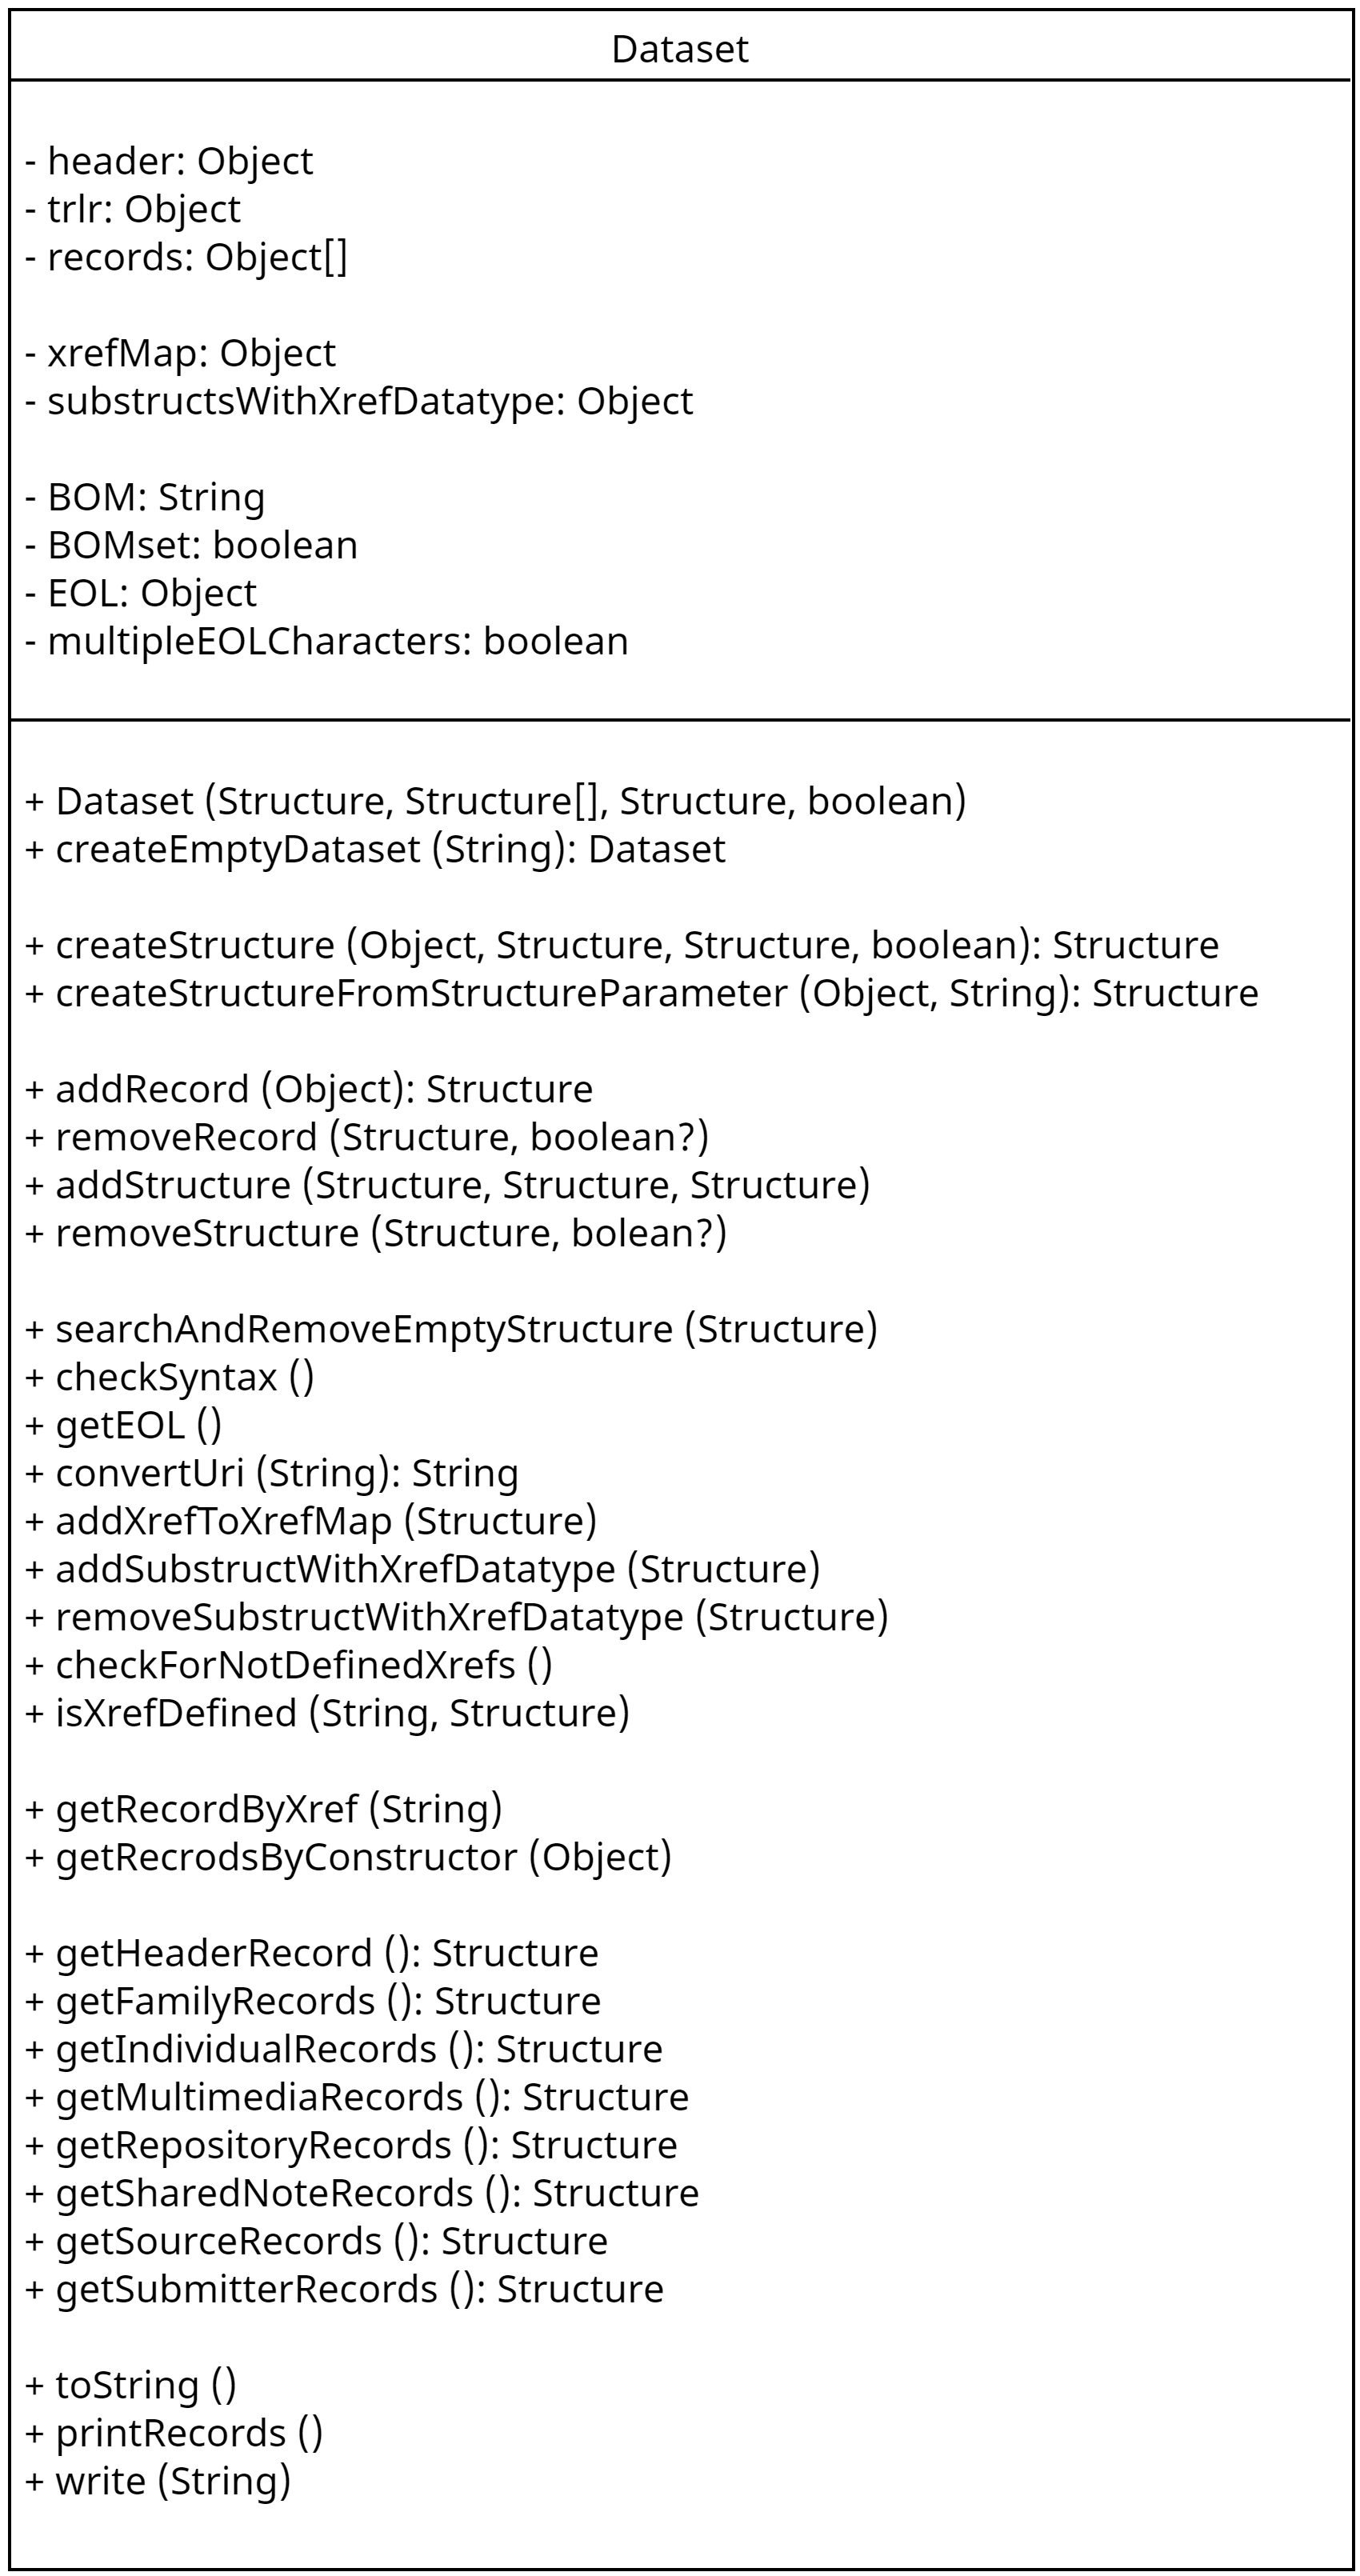
\includegraphics[width=0.65\textwidth]{images/UML_Class_Dataset.png}
	\caption{UML Klassendiagramm Dataset}
	\label{fig: UML Klassendiagramm Dataset}
\end{figure}


%========================================================================================
% SECTION: GEDCOM Parser
%========================================================================================
\section{Gedcom Parser}
\label{sec: Implementierung - Gedcom Parser}
Alle in dieser Arbeit vorgestellten Konzepte und Implementierungen werden im \textsc{Gedcom Parser} vereinigt, der die zentrale Klasse der Bibliothek \textit{gedcom7.js} darstellt. Die Klasse \textsc{GedcomParser} verfügt über die Methode \textit{parseGedFile} mit der Gedcom7 Dateien mit Hilfe der Node.js FileSystem Bibliothek als UTF-8 kodierte Zeichenkette eingelesen und anschließend mit der Methode \textit{parseString} geparsed werden kann. Wie im Konzept in Abschnitt \ref{sec: Konzept - Gedcom Parser} dargestellt, wird ein Nearley Parser erstellt für ein Dataset erstellt, der String geparsed und anschließend aus den extrahierten Informationen eine Instanz der Klasse \textsc{Dataset} erzeugt die zurückgegeben wird. Das Sequenzdiagramm dieser Methode ist in Abbildung \ref{fig: Sequenz Gedcom Parser} dargestellt.


Im folgenden wird ein beispielhafter Ablauf für die Verwendung der Bibliothek \textit{gedcom7.js} dargestellt. Dazu wird eine Gedcom7 Datei eingelesen, die den FamilyRecord aus Listing \ref{lst: family record example} enthält:

\vspace{1em}
{
\noindent
Im ersten Schritt wird die Gedcom7 Datei eingelesen, geparsed und in ein Dataset überführt. Dazu wird eine Instanz der Klasse \textsc{GedcomParser} erzeugt.
\begin{javascriptNoCaption}
	gedcomParser = new GedcomParser();
\end{javascriptNoCaption}
Anschließend wird der Pfad zur Gedcom7 Datei an die Methode \textit{parseGedFile} übergeben. In diesem Beispiel liegt die Datei im selben Verzeichnis, wie die ausgeführte JavaScript-Datei unter dem Namen ''FamilyExample.ged``. 
\begin{javascriptNoCaption}
	const dataset = await gedcomParser.parseGedFile('./FamilyExample.ged');
\end{javascriptNoCaption}
Dann kann die Family aus Listing \ref{lst: family record example} über den Cross-Reference-Identifier gesucht werden.
\begin{javascriptNoCaption}
	const famF1 = dataset.getRecordByXref('@F1@');
\end{javascriptNoCaption}
Sollen Informationen über die Kinder der Family ausgegeben werden, kann dies über 
\begin{javascriptNoCaption}
	const nchi = famF1.getChildrenInformation();
	console.log(nchi);
	// Ausgabe: 
	   {
		 numberOfChildren: 2,
		 type: null,
		 parentInformation: null,
		 eventDetails: null
	   }
\end{javascriptNoCaption}
realisiert werden. Außerdem kann das Datum der Hochzeit herausgefunden werden mit:
\begin{javascriptNoCaption}
	const marrInfo = famF1.getMarriageInformation();
	console.log(marrInfo.marriages[0].eventDetails.date);
	// Ausgabe: 
	   {
		 type: "DateValue"
		 date: 1951-03-01T00:00:00.000TZ
	   }
\end{javascriptNoCaption}
Soll nun die Information zum Family Record hinzugefügt werden, dass die Ehe wieder geschieden wurde, kann dies über die DIV-Structure ausgedrückt werden. Mit Hilfe der Methode \textit{addSubstructure} kann eine DIV-Structure zum Family Record hinzugefügt werden:
\begin{javascriptNoCaption}
	const div = {
		uri: 'g7:DIV',
		substructs: [{
			uri: 'g7:DATE',
			lineVal: '28 DEC 1963',
		}]
	};
	famF1.addSubstructure(div);
\end{javascriptNoCaption}
Wird der Family Record nun ausgegeben, ist die neue DIV-Structure in der Ausgabe mit korrekter Gedcom7 Line-Syntax enthalten:
\begin{javascriptNoCaption}
	console.log(famF1.toString());
	// Ausgabe: 
	   0 @F1@ FAM
	   1 HUSB @I1@
	   1 WIFE @I2@
	   1 MARR
	   2 DATE 1 MAR 1951
	   1 NCHI 2
	   1 DIV
	   2 DATE 28 DEC 1963
\end{javascriptNoCaption}
}

%========================================================================================
% SECTION: Test
%========================================================================================
\section{Test der Implementierung}
Die Implementierung der Bibliothek \textit{gedcom7.js} wurde im Entwicklungsprozess ausgiebig getestet. Mit Hilfe des in Kapitel \ref{sec: Mocha} vorgestellten JavaScript Test-Frameworks \textit{mocha} wurden insgesamt 176 Test spezifiziert, die die wichtigsten Use-Cases der Bibliothek abdecken. Im Besonderen wurden die Klassen \textsc{Gedcom Parser}, \textsc{Dataset}, \textsc{Structure} und \textsc{Family} getestet. Da der \textsc{Gedcom Parser} intern die vom \textsc{Grammar Generator} erstellte Nearley Grammatik verwendet, wird beim Test der \textsc{Grammar Generator} beim Test des \textsc{Gedcom Parser} indirekt mitgetestet. In zukünftigen Arbeiten sollten jedoch zusätzliche Tests für den Grammatik Generator implementiert werden, da eine korrekte Syntaxüberprüfung die Grundlage für eine fehlerfreie Nutzung der Bibliothek darstellt. Besonders wenn eine Schnittstelle zum \textsc{Grammar Generator} zur Erstellung von Extensions eingeführt wird, sind ausgiebige Testfälle unabdingbar. Außerdem sollten in zukünftigen Arbeiten Tests für die \textit{Datatype Structures} und alle weiteren Records implementiert werden. 


Im folgenden wird anhand eines exemplarischen Tests gezeigt, wie die Komponenten der Bibliothek \textit{gedcom7.js}getestet wurden. Zusätzlich zu \textit{Mocha} wurde dazu die \textit{Node.js} Assertion-Bibliothek \textit{Chai} verwendet, mit der ausdrucksstarke und leicht verständliche Testfälle in englischer Sprache definiert werden können. Als Testgrundlage wurden die 7 Gedcom7 Dateien verwendet, die von \textit{Family Search} als Beispieldateien bereitgestellt wurden. Diese Dateien decken die komplette Gedcom7 Spezifikation ab und versuchen alle Structuretypes, Datatypes und Sonderfälle abzudecken. Funktioniert das Parsen und Verarbeiten dieser Dateien korrekt, kann davon ausgegangen werden, dass die Gedcom7 Spezifikation korrekt in der Bibliothek abgebildet wurde.


Mit den in Listing \ref{lst: test lesen und schreiben gedcom7 dateien} aufgeführten Testfällen, wird das Lesen und Schreiben von Gedcom7 Dateien getestet. Dazu werden die oben angesprochenen, von \textit{Family Search} als Beispieldateien bereitgestellten, Gedcom7 Dateien mit einer Instanz des \textsc{Gedcom Parser} eingelesen und als \textsc{Dataset} zurückgegeben. Dieses Dataset wird über die Methode \textit{write()} temporär gespeichert und anschließend mit der ursprünglichen Gedcom7 Datei verglichen. Dieser Vergleich kann auf einfache Weise mit der Textvergleichsimplementierung \textit{diff}\footnote{Nähere Informationen sind unter https://www.npmjs.com/package/diff angegeben.} umgesetzt werden, mit der die Inhalte der Dateien Zeichen für Zeichen verglichen werden. 


Auf diese Weise wird ebenfalls sichergestellt, dass Gedcom7 Dateien die eingelesen aber unverändert bleiben, nach der Ausgabe identisch bleiben. Dies ist eine wichtige Anforderung, da textbasierte Dateiformate wie der Gedcom Standard gerne über Versionsverwaltung administriert werden. Für diesen Use-Case wäre es nicht annehmbar, wenn sich Änderungen in Dateien ergeben, die nicht angepasst wurden. Damit eine identische Ausgabe möglich ist, müssen im \hyperref[fig: UML Klassendiagramm Dataset]{\textsc{Dataset}} Angaben über die verwendeten EOL-Character und das Byte-Order-Mark gespeichert werden.

\begin{javascript}{Testfälle für das Lesen und Schreiben von korrekten Gedcom7 Dateien}{lst: test lesen und schreiben gedcom7 dateien}
	describe('test if gedcom file is equivalent before and after parsing', () => {
		const gedcomParser = new GedcomParser();
		const path = 'test/sampleData/ExampleFamilySearchGEDCOMFiles/';
		
		// Family Search Example Files
		const gedFiles = [
			'escapes.ged',
			'long-url.ged',
			'maximal70_without_extensions.ged',
			'minimal70.ged',
			'remarriage1.ged',
			'same-sex-marriage.ged',
			'voidptr.ged'
		];
		
		forEach(gedFiles)
		.it('#%s', async (fileName) => {
			// read Gedcom file as String
			const beforeParsing = await readGedFile(path + fileName);
			// parse Gedcom String and write it to temp.ged
			const dataset = gedcomParser.parseString(beforeParsing);
			await fs.writeFile(path + 'temp.ged', '');
			await dataset.write(path + 'temp.ged');
			// read temp.ged as String and compare it with original file
			const afterParsing = await readGedFile(path + 'temp.ged');
			
			// expect files to be equal
			expect(diffChars(beforeParsing, afterParsing)).to.have.lengthOf(1);
		});
	});
\end{javascript}

In der folgenden Auflistung sind alle weiteren Testfälle aufgeführt, die im Rahmen dieser Arbeit implementiert wurden. Alle Testfälle sind im Repository der Bibliothek im Ordner \textit{Test} abgelegt. 

\bgroup
\def\arraystretch{1.5}%  1 is the default, change whatever you need
\setlength{\tabcolsep}{18pt}
\begin{longtable}{|p{2cm}|p{10cm}|}
	\hline
	\textbf{Dataset} & { \vspace{-1.8em}
		\begin{itemize}
			\item Vergleich von geschriebenen Gedcom7 Dateien mit dem Original
			\item Suchen von Records im Dataset
			\item Fehler finden bei Eingabe von Gedcom7 Dateien mit nicht definiertem Xref
			\item Fehler finden bei Eingabe von Gedcom7 Dateien mit mehrfach verwendetem Xref
			\item Warnungsausgabe bei fehlendem Byte-Order-Mark
			\item Verwendung der richtigen EOL-Character
	\end{itemize}\vspace{-1.6em}}\\
	\hline
	\textbf{Parser} & { \vspace{-1.8em}
		\begin{itemize}
			\item Parsen von korrekten Gedcom7 Dateien ohne Fehler
			\item Syntaxfehler finden beim Parsen von Gedcom7 Dateien mit fehlerhafter Syntax
			\item Syntaxfehler finden beim Parsen von Gedcom7 Dateien mit fehlendem Header und/oder Trailer
		\end{itemize}\vspace{-1.6em}}\\
	\hline
	\textbf{Structure} & { \vspace{-1.8em}
		\begin{itemize}
			\item Finden von Substructures anhand des Tags
			\item Finden von Substructures anhand des LineValues
			\item Ändern des LineValues
			\item Ändern des Xref
			\item Hinzufügen von einer/mehrere Substructures mit keiner/einer/mehreren Substructures
		\end{itemize}\vspace{-1.6em}}\\
	\hline
	\caption{Bestandteile einer GEDCOM Line und ihre Bedeutung} % needs to go inside longtable environment
	\label{tab: gedcom line}
\end{longtable}
\egroup
\vspace{1em}
\chapter{Zusammenfassung und Ausblick}
\label{chap: Zusammenfassung und Ausblick}
In dieser Arbeit wurde ...




%------------------ Literaturverzeichnis & Index -------------------------------
\backmatter
\bibliography{literatur}								% Literaturverzeichnis (literatur.bib)


\printindex												% Index (optional)


%------------------ Anhänge ----------------------------------------------------
\begin{appendix}
	\chapter{Glossar}
\abbreviation{DSM}			{Distributed Shared Memory}
\abbreviation{AC}			{Atomic Consistency (dt.: Linearisierbarkeit)}
\abbreviation{RC}			{Release Consistency (dt.: Freigabekonsistenz)}
\abbreviation{SC}			{Sequential Consistency (dt.: Sequentielle Konsistenz)}
\abbreviation{WC}			{Weak Consistency (dt.: Schwache Konsistenz)}

	\chapter{Selbstständigkeitserklärung}
Ich erkläre hiermit, dass ich die vorliegende Seminararbeit ohne fremde Hilfe verfasst und nur die im Literaturverzeichnis angegebenen Quellen verwendet habe.

\vspace{3cm}

\begin{minipage}[t]{3cm}
	\rule{3cm}{0.5pt}
	Datum
\end{minipage}
\hfill
\begin{minipage}[t]{9cm}
	\rule{9cm}{0.5pt}
	Unterschrift der Kandidatin/des Kandidaten
\end{minipage}
	% Selbstständigkeitserklärung
\end{appendix}


\end{document}
